\documentclass[11pt,a4paper]{article}
\usepackage[margin=2.2cm]{geometry}
\usepackage[T1]{fontenc}
\usepackage{lmodern,microtype}
\usepackage{graphicx,booktabs,tabularx,float,caption,xcolor,enumitem,amsmath,array,longtable}
\usepackage{flafter}
\usepackage[section]{placeins}
\usepackage{tikz}
\usetikzlibrary{arrows.meta,positioning,fit,calc}
\usepackage[hidelinks]{hyperref}
\graphicspath{{../figures/}{../../results/plots/}}
\captionsetup{font=small,labelfont=bf}
\setlist{itemsep=2pt,topsep=4pt}
\setlength{\parskip}{4pt}
\newcolumntype{L}{>{\raggedright\arraybackslash}X}
\newcolumntype{R}{>{\raggedleft\arraybackslash}X}
\newcommand{\key}[1]{\par\smallskip\noindent\colorbox{black!6}{\parbox{\dimexpr\linewidth-2\fboxsep}{\small\textbf{Key idea.} #1}}\par\smallskip}
\newcommand{\code}[1]{\texttt{#1}}
\renewcommand{\floatpagefraction}{0.75}

\title{\textbf{GeoGuessers: What We Did, Why, and What It Means}\\[4pt]
\large Internal report for the team (not for submission)\\[2pt]
\normalsize Phases 0--4 complete; Phase 5 designed. Read this before the presentation.}
\author{Swayam Goyal (2024111012) \quad Siddharth Choudhary (2024111021)\\ Yakkala Viswanadha Kartikeya (2024111033)}
\date{}

\begin{document}
\maketitle
\tableofcontents
\newpage

%=====================================================================
\section{The project in one page}
\paragraph{The question.} Our professor asked us to work like a systems team: take a very large, high-resolution
DEM (Himalaya, 90\,m down to 1\,m), use only a laptop, and find out (a) where today's standard tools (GDAL, QGIS)
stop being practical and \emph{why}: what is the real bottleneck (disk, RAM, CPU, GPU transfer, rendering)? And (b)
how to process and display only what the user is looking at, using a \textbf{pyramid} (the same DEM stored at several
resolutions), computing slope / aspect / hillshade \textbf{on demand}, and using the CPU and GPU where each really
helps. Our literature review turned this into these research gaps:
\begin{itemize}
  \item[\textbf{G1}] No study reports where standard GDAL/QGIS terrain tools stop being practical on one laptop,
  separated into stages (read, compute, CPU$\leftrightarrow$GPU transfer, write, display).
  \item[\textbf{G2}] No study computes terrain derivatives on demand from pyramid levels, or measures how wrong a
  coarse-level slope is against the time it saves.
  \item[\textbf{G3}] (stretch) Accuracy of fast approximate viewshed (XDraw) vs exact R3 in high relief; A* vs Dijkstra.
\end{itemize}

\paragraph{What is finished.} Phase 0 (setup), Phase 1 (data), Phase 2 (baseline of the standard tools, E1/E2/QGIS),
Phase 3 (our own CPU and GPU engine, E3/E4), Phase 4 (derivatives on demand from the pyramid, E5). Every result was
audited number by number against the raw data. Phase 5 (the interactive viewer) is designed but not started.

\paragraph{The answer, in six lines.}
\begin{enumerate}
  \item \code{gdaldem} (GDAL's terrain tool, which QGIS also calls) \textbf{never runs out of memory}: it handles
  10.8 billion cells (43\,GB) with 0.87\,GB of RAM. It just gets slower: 3.5\,min for one slope pass at 1\,m.
  \item Its bottleneck is \textbf{computation on a single CPU thread} (73\% of the time; 1 of 22 threads used).
  \item For \textbf{display}, the bottleneck is \textbf{reading full-resolution data}: without a pyramid QGIS needs
  32\,s to draw the whole 1\,m area; with a pyramid 0.09\,s at any size.
  \item \textbf{Our CPU engine} computes slope \textbf{2.1--3.5$\times$ faster} than \code{gdaldem} on the same cores
  (1\,m: 60\,s vs 208\,s), identical results, memory flat at $\sim$1.4\,GB. Loading the whole grid into RAM (the naive
  way) breaks above roughly 0.5--0.7 billion cells.
  \item \textbf{Our GPU kernel} computes 50$\times$ faster than the CPU kernel, but the run is only 1.0--1.4$\times$
  faster (1\,m: 44\,s): 95\% of the GPU's own time is copying, and the run is limited by decompressing the input and
  writing the output. \textbf{The bottleneck moved from computation to data movement.}
  \item \textbf{On demand from the pyramid}, one display tile costs 5--8\,ms at every zoom level, 8--450$\times$ less
  than computing it exactly at full resolution. The price: slope comes out \emph{too low}, by 2.3$^\circ$ RMSE one
  level up to 6.4$^\circ$ four levels up (worst on steep slopes). Aspect is barely affected.
\end{enumerate}

\paragraph{Where we go next.} Phase 5: a viewer where the user sees the whole map, drags a bounding box, and only
that box is computed at the right pyramid level (Section~\ref{sec:phase5}). Then the final report and demo.

\begin{figure}[!htbp]
\centering
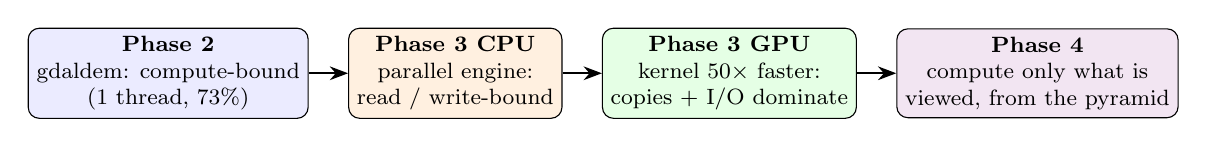
\begin{tikzpicture}[font=\footnotesize, box/.style={draw, rounded corners, align=center, minimum height=9mm, inner sep=3pt},
  arr/.style={-{Stealth}, thick}]
\node[box, fill=blue!8] (p2) {\textbf{Phase 2}\\gdaldem: compute-bound\\(1 thread, 73\%)};
\node[box, fill=orange!12, right=5mm of p2] (p3) {\textbf{Phase 3 CPU}\\parallel engine:\\read / write-bound};
\node[box, fill=green!10, right=5mm of p3] (p3g) {\textbf{Phase 3 GPU}\\kernel 50$\times$ faster:\\copies + I/O dominate};
\node[box, fill=violet!10, right=5mm of p3g] (p4) {\textbf{Phase 4}\\compute only what is\\viewed, from the pyramid};
\draw[arr] (p2) -- (p3); \draw[arr] (p3) -- (p3g); \draw[arr] (p3g) -- (p4);
\end{tikzpicture}
\caption{The story of the project in one picture. Each step removes the current bottleneck and exposes the next one.
The answer to ``how do we handle a DEM bigger than RAM on a laptop'' is: do not process all of it; read and compute only
the window and resolution the user needs.}
\end{figure}

%=====================================================================
\section{Concepts you need (glossary)}
\begin{longtable}{>{\raggedright\arraybackslash}p{3.4cm}>{\raggedright\arraybackslash}p{12.0cm}}
\toprule
Term & Meaning, and why it matters for us \\
\midrule
\endhead
\multicolumn{2}{l}{\textit{Data and formats}} \\
DEM & Digital Elevation Model: a grid (raster) where each cell stores a ground height. \\
Resolution vs cells & Halving the cell size quadruples the number of cells. Our area at 8\,m is 169\,M cells; at 2\,m
2.7\,B; at 1\,m 10.8\,B. Run time follows the number of cells, which is why we talk in cells, not metres. \\
float32 / float64 & 4 / 8 bytes per number. 10.8\,B cells $\times$ 4\,B = 43\,GB, 2.6$\times$ our 16\,GB RAM. float32 is
what the files store; float64 is more precise arithmetic. \\
MB vs MiB & MB = $10^6$ bytes, MiB = $2^{20}$ (5\% more). Our harness records MiB; our documents use MB/GB. GPU memory
is given in MiB/GiB as the driver reports it. (Mixing these was one of the audit fixes.) \\
CRS, UTM 44N & Coordinate reference system. Slope needs the cell size in metres, so everything is reprojected to UTM
zone 44N (EPSG:32644). Degrees would give wrong slopes. \\
Resampling & Moving a grid onto a new grid. \emph{Nearest} copies the closest value (keeps values, blocky),
\emph{bilinear}/\emph{cubic} blend neighbours (smooth), \emph{average} averages all cells that fall into a coarser cell
(used to build pyramids). \\
GeoTIFF, strips, tiles & The file format. Data stored in rows (strips) or squares (tiles, e.g.\ 512$\times$512). Tiles
let a program read a small window without reading whole rows. \\
Compression, predictor & LZW, DEFLATE, ZSTD shrink the file; the price is CPU time to decompress on every read. The
floating-point predictor (=3) makes height data compress much better. \\
COG & Cloud-Optimized GeoTIFF: a tiled GeoTIFF with its pyramid stored inside. All our prepared grids are COGs
(512 tiles, ZSTD). \\
Overview / pyramid level & A coarser copy stored inside the file. Level $k$ has cell size $\approx 2^k \times$ base
(2\,m $\to$ 4, 8, 16\,\dots\,m). GDAL halves the size and rounds down, so when the grid size is not divisible by $2^k$
a level cell is slightly bigger than $2^k$ fine cells (8.002 instead of 8). \\
Vertical datum & What height zero means. HMA 8\,m and Chamoli 2\,m use the WGS84 ellipsoid; Copernicus the EGM2008
geoid: about 24.5--26\,m apart here. A constant offset does not change slope, but matters for viewsheds. \\
NMAD & Normalised median absolute deviation: a robust standard deviation used to compare DEMs. \\
Synthetic grid & Our 2\,m and 1\,m grids of the whole area are \emph{cubic upsamples} of the 8\,m DEM. They have the right
size but no real extra detail: used for timing only, never accuracy. \\
\midrule
\multicolumn{2}{l}{\textit{Terrain operators}} \\
3$\times$3 operators & Slope, aspect, hillshade, TRI, TPI, roughness each look at a cell and its 8 neighbours. One
visit per cell: O(N). Faster versions differ in implementation, not in the maths. \\
Horn vs ZT & Two ways to estimate the height gradient (Section~\ref{sec:formulas}). Horn uses all 8 neighbours with
weights; Zevenbergen--Thorne only the 4 direct ones. GDAL's default is Horn. \\
Slope / aspect / hillshade & Steepness in degrees; direction the slope faces (0--360$^\circ$ from north); shaded relief
lit by a sun at azimuth 315$^\circ$, altitude 45$^\circ$ (grey value 1--255, 0 = nodata). \\
TRI, TPI, roughness & Terrain Ruggedness Index (Riley: root of summed squared differences; Wilson: mean absolute
difference), Topographic Position Index (cell minus mean of neighbours), max $-$ min of the window. \\
Nodata & Cells without a value ($-9999$). An operator output is nodata if any of the 9 window cells is nodata;
\code{gdaldem} also leaves the outer ring of the grid empty. \\
\midrule
\multicolumn{2}{l}{\textit{Measurement}} \\
File cache, cold / warm & Windows keeps recently read file data in spare RAM (the standby list). Cold: we empty it
first, so the file must come from disk. Warm: immediate repeat, data may come from RAM. \\
Peak working set & The most RAM a process held at any moment: our ``peak memory''. \\
ns per cell & Run time / number of cells, in nanoseconds: makes grids of different sizes comparable. \\
Median, IQR, spread & We repeat runs and report the median (robust to one odd run). IQR = 75th $-$ 25th percentile;
spread = (max $-$ min) / median. \\
Warm-up run & rep 0: a first run that is thrown away (loads programs and caches). \\
P-, E-, LP-cores & Our CPU has 6 fast performance cores (12 threads), 8 slower efficiency and 2 very slow low-power cores.
Where Windows puts a process changes its speed by up to 2.7$\times$; we pin tools to the P-cores. \\
Turbo budget & Cores share a power/heat budget: if other cores are busy, the active core clocks lower. \\
Defender scan, \code{\$Deleted} & Windows Defender scans new files; a file deleted while being scanned keeps its space
reserved in a hidden NTFS area until the scan ends. \\
Stage split & Dividing a run into read / compute / write (or copy / kernel for the GPU) to see where time goes. \\
Amdahl's law & If a part $p$ of a run is sped up infinitely, the whole run speeds up at most $1/(1-p)$. Read + write =
27\% of gdaldem $\Rightarrow$ parallelising only compute gives at most $\sim$3.7$\times$. \\
Read-bound / write-bound & The run's speed is set by reading (decompressing) input or writing output, not by
computation. \\
\midrule
\multicolumn{2}{l}{\textit{Our engine (CPU)}} \\
Window, halo & The grid is processed in 2048$\times$2048 windows; each is read with a 1-cell border (halo) so the
3$\times$3 operators are exact at window edges. \\
Pipeline & Three stages that overlap: reader threads decode windows, the main thread computes, one writer thread
writes. Bounded queues (at most 6 windows in flight) keep memory flat. \\
Numba, JIT, \code{prange} & Numba compiles a Python loop to machine code just in time; \code{prange} splits the rows
over all cores. The compiled kernel is cached on disk. \\
Fused kernel & Slope, aspect and hillshade computed from one gradient pass: three products for little more than one. \\
Naive version & Read the whole grid into memory and compute with NumPy: simple, but needs $\sim$24 bytes per cell. \\
\midrule
\multicolumn{2}{l}{\textit{Our engine (GPU)}} \\
CUDA kernel, CuPy & A function run by thousands of GPU threads at once (one per cell). We write the kernels in CUDA C
and compile them through CuPy at run time. \\
H2D / D2H, PCIe & Copies host$\to$device and device$\to$host over the PCIe bus (here 4.0 $\times$8). Moving a cell in and
out costs $\sim$0.9\,ns; computing it 0.04\,ns. \\
Pinned memory & Page-locked host memory: copies run at full PCIe speed and can overlap with kernels. \\
CUDA streams & Independent queues of GPU work; with 2 streams the copies of one window overlap the kernel of the next. \\
Crossover & The window size above which the GPU (including copies) beats the CPU: $512^2$ cells for slope. \\
VRAM, TDR & GPU memory (8\,GiB, we capped use at 4\,GiB); TDR is Windows' 2\,s GPU watchdog (our kernels take ms). \\
\midrule
\multicolumn{2}{l}{\textit{Phase 4 (pyramid)}} \\
On demand & Compute the derivative from the pyramid level being displayed, at that level's cell size. \\
Truth (E5) & Slope computed at full resolution, then averaged over exactly the fine cells a coarse cell covers. \\
Footprint & The fine cells covered by one coarse cell (those whose centres lie inside it). \\
Bias, RMSE, MAE & Mean of (on demand $-$ truth); root mean squared error; mean absolute error. Negative bias = too low. \\
Fully valid cell & A coarse cell whose footprint and 8 neighbours contain no nodata: the only cells we score. \\
Circular mean, $R$ & Average of directions (via sin/cos); $R$ (0--1) says how much the directions agree. \\
Levels up & How many pyramid levels above the source data: the error depends on this, not on metres. \\
\midrule
\multicolumn{2}{l}{\textit{Experiments}} \\
E1--E6 & E1 gdaldem baseline; E2 storage layouts; E1q QGIS display; E3 CPU engine; E4 GPU engine; E5 pyramid accuracy
and time; E6 interactive viewer (Phase 5, not yet run). \\
\bottomrule
\end{longtable}

\subsection{The terrain operators and their formulas}\label{sec:formulas}
Label the 3$\times$3 window around cell $e$ as
\[
\begin{array}{ccc} a & b & c\\ d & e & f\\ g & h & i \end{array}
\qquad \text{cell size } \Delta x = \Delta y .
\]
\textbf{Horn (1981):}
\[ \frac{\partial z}{\partial x} = \frac{(c+2f+i)-(a+2d+g)}{8\Delta x},\qquad
\frac{\partial z}{\partial y} = \frac{(a+2b+c)-(g+2h+i)}{8\Delta y}. \]
\textbf{Zevenbergen--Thorne (1987):}
\[ \frac{\partial z}{\partial x} = \frac{f-d}{2\Delta x},\qquad \frac{\partial z}{\partial y} = \frac{b-h}{2\Delta y}. \]
Then
\[ s = \arctan\sqrt{(\partial z/\partial x)^2 + (\partial z/\partial y)^2}, \qquad
\text{aspect} = \operatorname{atan2}\!\left(-\tfrac{\partial z}{\partial x}, -\tfrac{\partial z}{\partial y}\right) \]
(\textbf{slope} $s$; \textbf{aspect} is the direction of steepest descent in degrees from north, nodata on perfectly flat
cells); \textbf{hillshade} (sun azimuth $\phi$, altitude $\theta$):
$\cos\gamma = \sin\theta\cos s + \cos\theta\sin s\cos(\phi - \text{aspect})$, value $= 1 + 254\max(\cos\gamma, 0)$, as
\code{gdaldem} does; \textbf{TRI} (Riley) $= \sqrt{\sum (z_n - z_e)^2}$, (Wilson) the mean of $|z_n - z_e|$ over the 8
neighbours $n$; \textbf{TPI} $= z_e - \text{mean}(z_n)$; \textbf{roughness} $= \max - \min$ of the window.

Three consequences used later: (1) every operator divides by the cell size, so slope computed on a coarser pyramid
level is \emph{different} (smoother), not just faster: that is what E5 measures. (2) All six need the same few
neighbour differences, so computing them together (one pass) shares most of the work. (3) \code{gdaldem} adds the
neighbour values in float32; our float64 engine therefore differs from it by tiny rounding on nearly flat cells.

\subsection{Error measures used in Phase 4}
For the $n$ scored cells with on-demand value $c_j$ and truth $t_j$:
$\text{bias} = \frac1n\sum (c_j - t_j)$, $\text{MAE} = \frac1n\sum |c_j - t_j|$,
$\text{RMSE} = \sqrt{\frac1n\sum (c_j - t_j)^2}$. Aspect differences are taken around the circle
($\min(|\Delta|, 360-|\Delta|)$).

%=====================================================================
\section{What we did, in order}
\subsection{Phases 0--2 (setup, data, baseline)}
\begin{enumerate}
\item \textbf{Setup.} Python environment \code{geo} (GDAL 3.13.3, rasterio, Numba, CuPy 14.2, FastAPI) via Miniforge at
\code{D:\textbackslash miniforge3} (the default path failed because our user folder name has a space), QGIS 3.44.14.
Checked: CuPy runs on the RTX 4060; QGIS slope matched an OpenTopography reference to $10^{-5}$ degrees.
\item \textbf{Choosing data.} The first downloads (an Everest 90\,m crop, two single 8\,m strips) were too small or
patchy. We switched to the NASA High Mountain Asia 8\,m \emph{mosaic} tile-571 (Uttarakhand), downloaded Copernicus
30\,m and 90\,m for the same box through the OpenTopography API, and found a free real 2\,m DEM of the Chamoli valley
inside the tile (Bhushan \& Shean, Zenodo).
\item \textbf{One area, many resolutions.} Run time depends on the number of cells, not on which mountain it is. One
area means grid size is the only thing that changes, and the real 2\,m data gives a ``truth'' for accuracy.
\item \textbf{Checking the data.} Tile-571 is 90.4\% valid (gaps in the south-east). The 8\,m tile is 24.5\,m below
Copernicus (datum). Chamoli 2\,m averaged to 8\,m matches the 8\,m DEM to a median of $-0.7$\,m (NMAD 5.1\,m). Chamoli
was re-gridded with nearest-neighbour (only 0.09/0.16\,m off our grid), so its heights are untouched.
\item \textbf{Are synthetic grids OK?} No free 1\,m DEM exists here. On a 16\,M-cell crop, an 8\,m grid rebuilt from
16\,m takes the same gdaldem time as the real one, but its slopes are off by 2.3--3.0$^\circ$ RMSE, and nearest-neighbour
data compresses 26\% better (fake fast reads). Decision: synthetic 2\,m and 1\,m, \emph{cubic}, timing only.
\item \textbf{Building the harness} (Section~\ref{sec:harness}): exact per-process measurements, cold-cache flushing,
resumable sweeps.
\item \textbf{First E1 pass} (74 min, 560 runs, 0 failures), then a critical review: the ``read'' reference was wrong,
one run was a 2$\times$ outlier, conditions were not recorded.
\item \textbf{Fixing the method.} Core test $\to$ pin to performance cores. New pure read reference. Defender's CPU use
measured (tiny). Run conditions saved with every sweep.
\item \textbf{Second attempt} ran into a full disk: 108\,GB of deleted outputs held in \code{\$Deleted} while Defender
scanned them. We stopped, freed space, added a safeguard (wait until deleted space is released), re-ran.
\item \textbf{Chamoli anomaly.} Some runs 25--35\% slower in streaks, with foreign disk reads: background scanning of
previous outputs. Then E2 (10.8\,GB outputs) was stopped by the safeguard itself (35.6\,GB held $>$15 min).
\item \textbf{Final setup, clean re-run.} Only the two scratch folders excluded from Defender, laptop restarted, everything
re-run: \textbf{832 runs, 0 failures}. Disturbed attempts kept as evidence. GDAL tuning check afterwards
(\code{GDAL\_NUM\_THREADS}, bigger cache): no speed-up, so the baseline is \code{gdaldem} at its fastest.
\end{enumerate}

\subsection{Phase 3 (our engine)}
\begin{enumerate}
\setcounter{enumi}{11}
\item \textbf{Kernels and correctness first.} NumPy reference kernels for all 10 configurations, then a parallel Numba
kernel (slope/aspect/hillshade fused). 60 tests against \code{gdaldem} on two $1024^2$ crops (one with 55\% nodata, one
steep). Found that \code{gdaldem} adds the Horn neighbours in float32; with that reproduced, every cell matched.
\item \textbf{First engine version}, then three fixes before benchmarking: it submitted all window reads at once (up to
$\sim$86\,GB in memory at 1\,m) $\to$ bounded prefetch; rasterio's ``boundless'' read was slow $\to$ manual padding
(8\,m slope 1.55\,s $\to$ 1.12\,s); writing in the compute thread blocked the kernel $\to$ one writer thread (as the GDAL
multi-threading docs advise). Also: Numba used 22 threads while the process was pinned to 12 $\to$ explicit thread count.
\item \textbf{E3 sweep} (CPU, 347 runs), keeping the D: drive safe: outputs written to the internal SSD
and deleted after each run (max one run's output at a time, worst 97\,GB). Window-size sweep (84 runs) added because
the plan listed tile size. Diagnostics (kernel alone in memory, reader threads) as one-off scripts.
\item \textbf{Consolidation:} the 7 remaining \code{gdaldem} configurations benchmarked (154 runs, total E3 = 501) and a
full-grid correctness check (every cell of the whole 8\,m and 2\,m grids).
\item \textbf{GPU part} (with the explicit rule not to stress the laptop): CUDA kernels for all 10 configurations,
pinned buffers, 2 streams, CUDA-event timing, a 4\,GiB memory cap, and a temperature guard in the harness (wait below
75\,$^\circ$C, stop at 85\,$^\circ$C). E4 sweep 484 runs (0 failures, max 63\,$^\circ$C) plus a crossover test.
\end{enumerate}

\subsection{Phase 4 (pyramid on demand)}
\begin{enumerate}
\setcounter{enumi}{16}
\item \textbf{Discovered} that GDAL's overviews are not exact halvings on our grids (rounding), so a coarse cell's
footprint is taken from its geometry; \code{demlab/pyramid.py} with 11 tests.
\item \textbf{E5 accuracy:} slope and aspect from every overview level vs the full-resolution truth, on both real DEMs,
fully valid cells only; exact power-of-two pyramid as a cross-check; slope classes; thresholds; independent DEMs.
\item \textbf{E5 timing:} one display tile and the whole grid per level, three routes (on demand / full resolution /
precomputed), cold and warm, in one long-running process. Precomputed slope pyramids built and costed.
\end{enumerate}

\subsection{Audit, reports, plan change and hand-off}
\begin{enumerate}
\setcounter{enumi}{19}
\item \textbf{Full audit of Phases 2--4:} raw data integrity (1817 runs, no duplicates, only 2 expected failures), every
report regenerated (identical), every number in every document checked by independent read-throughs. Fixed: a table
that mixed cold and warm runs, MiB/GB units, several overstated claims (Section~\ref{sec:problems}). Added: correctness
check on the 90\,m/30\,m grids (the plan's ``correctness gate''), median + IQR for every configuration, stage chart.
\item \textbf{LaTeX progress reports} for Phases 3 and 4 (Phase 2 report corrected).
\item \textbf{Team decision for Phase 5:} zoom by bounding boxes instead of streaming tiles (Section~\ref{sec:phase5}).
\item \textbf{Hand-off:} everything pushed to GitHub; a complete SHA-256-verified copy (project, all data, environment,
notes) on the external drive \code{K:\textbackslash spatial project\textbackslash GeoGuessers\_handoff}.
\end{enumerate}

%=====================================================================
\section{The data}
\begin{figure}[!htbp]
\centering
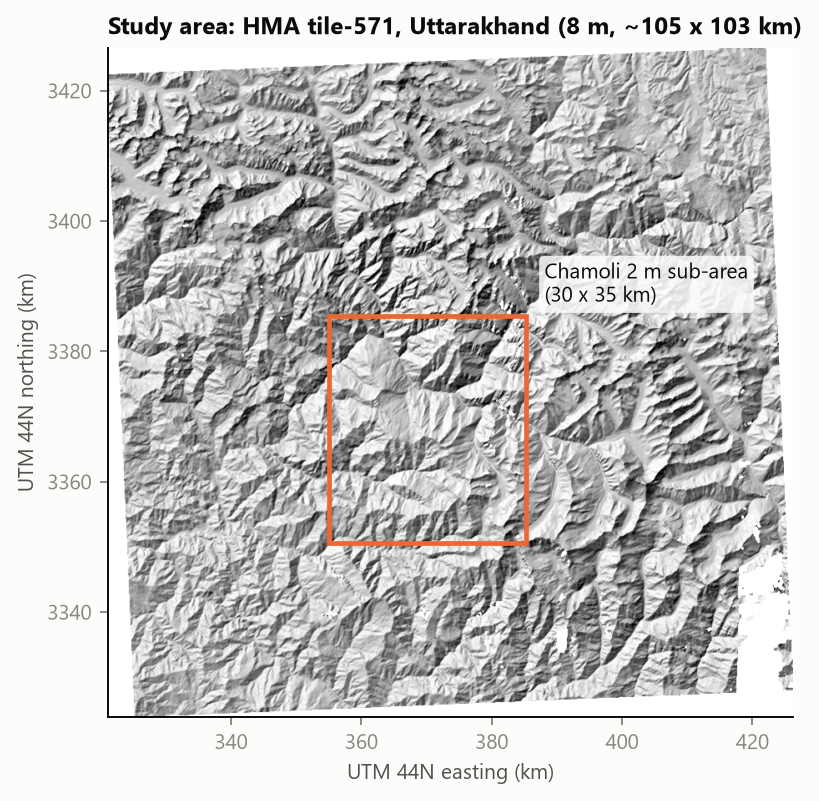
\includegraphics[width=0.5\linewidth]{study_area.png}
\caption{Study area (8\,m shaded relief) and the Chamoli 2\,m sub-area.}
\end{figure}
\begin{table}[!htbp]
\centering\small
\begin{tabularx}{\linewidth}{llrrL}
\toprule
File (\code{D:\textbackslash geoguessers\_data}) & Res. & Cells & Valid & Notes \\
\midrule
\code{prepared/tile571\_90m.tif} & 90\,m & 1.3\,M & 100\% & Copernicus GLO-90 \\
\code{prepared/tile571\_30m.tif} & 30\,m & 12\,M & 100\% & Copernicus GLO-30 \\
\code{prepared/tile571\_8m.tif} & 8\,m & 169\,M & 84\% & HMA mosaic; reprojection leaves thin empty wedges at the tilted edges \\
\code{prepared/chamoli\_2m.tif} & 2\,m & 264\,M & 94\% & real 2\,m; heights identical to the download; accuracy truth \\
\code{synthetic/tile571\_2m\_cubic.tif} & 2\,m & 2.7\,B & $\sim$89\% & timing only, 5.3\,GB on disk \\
\code{synthetic/tile571\_1m\_cubic.tif} & 1\,m & 10.8\,B & $\sim$89\% & timing only, 17.9\,GB on disk (incl.\ pyramid) \\
\bottomrule
\end{tabularx}
\end{table}
All grids share one origin on a 360\,m lattice (divisible by 90, 30, 8, 2 and 1), so they line up exactly. The raw
downloads are in \code{datasets/}; everything is listed with checksums in \code{datasets/manifest.csv} and rebuilt by
\code{python datasets/prepare.py [-{}-synthetic]}. Other data folders: \code{e2/} (8\,m layout copies; the 2\,m ones are on
the external drive), \code{bench\_out/} (scratch; holds the Phase 4 slope pyramids), \code{test\_fixtures/} (unit-test
crops), \code{tools/} (RAMMap).

%=====================================================================
\section{How the measurements work}\label{sec:harness}
\subsection{One run}
\code{bench/harness.py} starts the tool (e.g.\ \code{gdaldem slope in.tif out.tif}, or \code{python -m demlab.cli \dots}
for our engine) as its own process, pinned to a set of cores, and waits. When it ends, the harness reads from Windows,
for that process only: wall time, peak memory, total CPU time (so CPU time / wall time = average cores used), bytes
read and written. It also counts bytes physically read from the disks: if the disk read much more than the process
did, someone else was using the disk (our ``foreign disk read'' interference signal). Our engine additionally prints its
own stage timings (read wait, compute, write wait, writer busy; GPU copy/kernel times) as JSON, which go into the
\code{extra} column. One row per run in \code{results/runs.csv}. An early version sampled counters every 50\,ms and missed
the end of short runs; reading exact totals from the finished process fixed that.

\subsection{Cold cache}
Emptying the Windows file cache needs admin rights, so a scheduled task (\code{GeoGuessers-FlushCache} in the
\code{\textbackslash GeoGuessers} folder of the Task Scheduler) runs Sysinternals \code{RAMMap -Et} with admin rights; the benchmark triggers it without being admin. Verified: after a flush the whole file is read from disk again.
(An early mistake used \code{-Ec}, which is not a RAMMap option.)

\subsection{Protocol}
Real grids: 5 cold runs (cache emptied before each), then 1 warm-up and 5 warm runs. Synthetic 2\,m/1\,m: 3 cold + 1
warm (saved $\sim$5 hours; operator comparisons do not depend on size, so they come from the real grids). Medians are
reported; median and IQR of every configuration are in \code{results/run\_stats.md} (median IQR 1.2--1.6\% of the
median for E1--E4). Plugged in, Balanced power plan, Defender on (only scratch folders excluded), recorded per sweep in
\code{results/env/}.

\subsection{Why we pin to performance cores}
The same 8\,m slope job pinned to each of the 22 logical CPUs: performance cores 3.7--4.1\,s, efficiency cores
$\sim$6.6\,s (1.7$\times$), low-power cores up to 10.5\,s (2.7$\times$). Unpinned, Windows may move a background process
onto slow cores mid-run (one first-pass run took 108.9\,s instead of $\sim$56\,s). Pinning runs every baseline tool at its
best, so our speed-ups are \emph{conservative}. Our engine was measured both on the same 12 P-core threads (fair
comparison) and on all 22.

\subsection{Why only two folders are excluded from Defender}
Defender's CPU use during a run is tiny (0.02--0.05 core). The problem is \emph{after} the run: it scans each new
10--40\,GB output, and a file deleted meanwhile keeps its space reserved until the scan ends. That filled the disk once
(108\,GB) and slowed later runs. Excluding just our two scratch folders loses no protection. The harness also waits until
deleted space is released before the next run and stops cleanly if that takes more than 15 minutes.

\subsection{Splitting a gdaldem run into stages}
Two reference runs per grid: \textbf{read} (\code{bench/read\_blocks.py}: read and decompress every block, nothing else)
and \textbf{copy} (\code{gdal\_translate} to an uncompressed GeoTIFF: same read plus same-size write). Then write + tool
overhead $\approx$ copy $-$ read, and compute $\approx$ gdaldem $-$ copy. (The first read reference, \code{gdalinfo
-checksum}, spent half its time computing the checksum.)

\subsection{GPU safety}
Our rule was not to put the graphics card or the laptop at risk. So: CUDA kernels only through CuPy (no clock,
power-limit, fan or driver changes); GPU memory capped at 4\,GiB; before every GPU run the harness reads the GPU
temperature and waits until it is below 75\,$^\circ$C, and stops the sweep if a run ends at 85\,$^\circ$C or more; every
kernel is milliseconds, far below the 2\,s Windows watchdog. Result: max 63\,$^\circ$C, median 58\,$^\circ$C, max 2.0\,GiB.

\subsection{Experiments}
\begin{longtable}{>{\raggedright\arraybackslash}p{2.4cm}>{\raggedright\arraybackslash}p{13.0cm}}
\toprule
Experiment & What was run \\
\midrule
\endhead
E1 (560 runs) & 10 \code{gdaldem} configurations on 6 grids, cold and warm, plus read/copy references. At 1\,m only slope and
hillshade (Horn). \\
E2 (224 runs) & 7 storage layouts of the 8\,m and 2\,m grids: time to write, pure read, \code{gdaldem} slope. \\
E1q (48 runs) & QGIS (headless) opens the layer and draws one 1920$\times$1080 image, whole area or zoomed, with or without
the pyramid. \\
E3 (501 runs) & CPU engine, 24 variants on 8\,m / 2\,m real / 2\,m / 1\,m synthetic: 22 vs 12 threads; all 10 configurations;
fused products; with/without writing; compressed output; 1--22 threads; windows 512--8192; single-threaded NumPy kernel;
naive whole-grid NumPy. \\
E4 (484 runs) & GPU engine, same grids: optimisation steps (CuPy port $\to$ own kernel $\to$ pinned $\to$ 2 streams), float32
vs float64, all operators, fused products, windows, 4 vs 8 readers. Plus a crossover test (one in-memory window,
$128^2$--$8192^2$). \\
E5 & Accuracy of slope/aspect from every pyramid level (Chamoli 2\,m: 6 levels; 8\,m: 5 levels) on fully valid cells,
exact-pyramid cross-check, slope classes, thresholds, independent DEMs. Timing: one $512^2$ tile at 8 places and the
whole grid per level, three routes, cold/warm (670 timings summarised). \\
\bottomrule
\end{longtable}

%=====================================================================
\section{Phase 2 results: the standard tools}
\subsection{E1: how gdaldem scales}
\begin{figure}[!htbp]
\centering
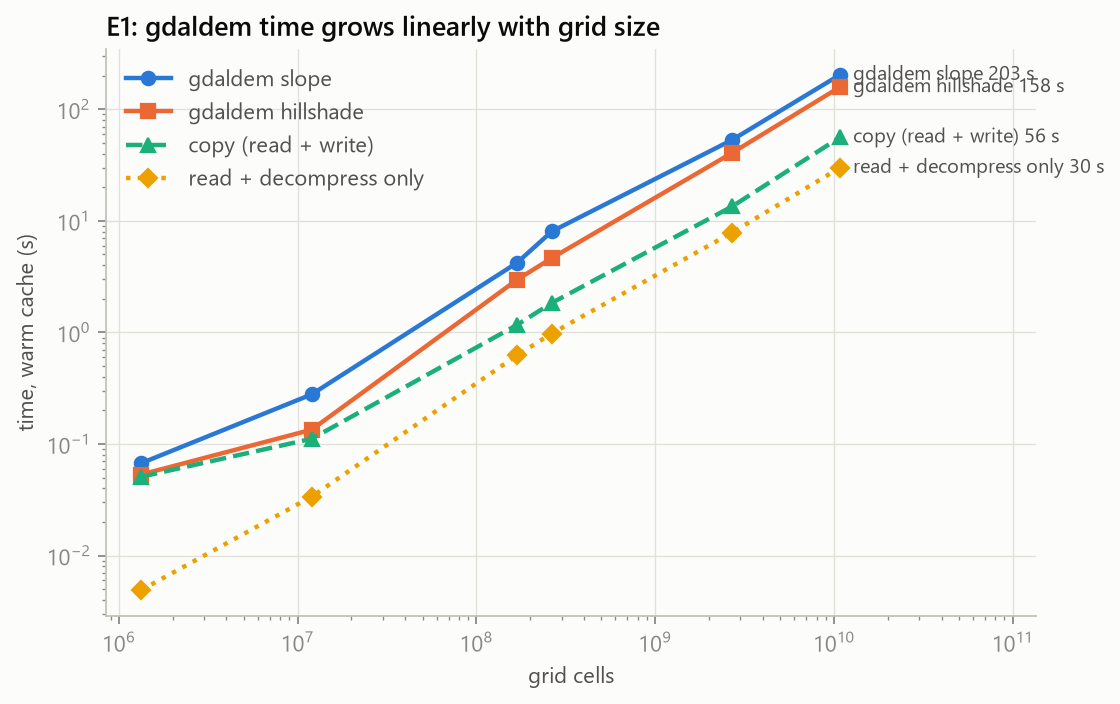
\includegraphics[width=0.49\linewidth]{e1_scaling.png}\hfill
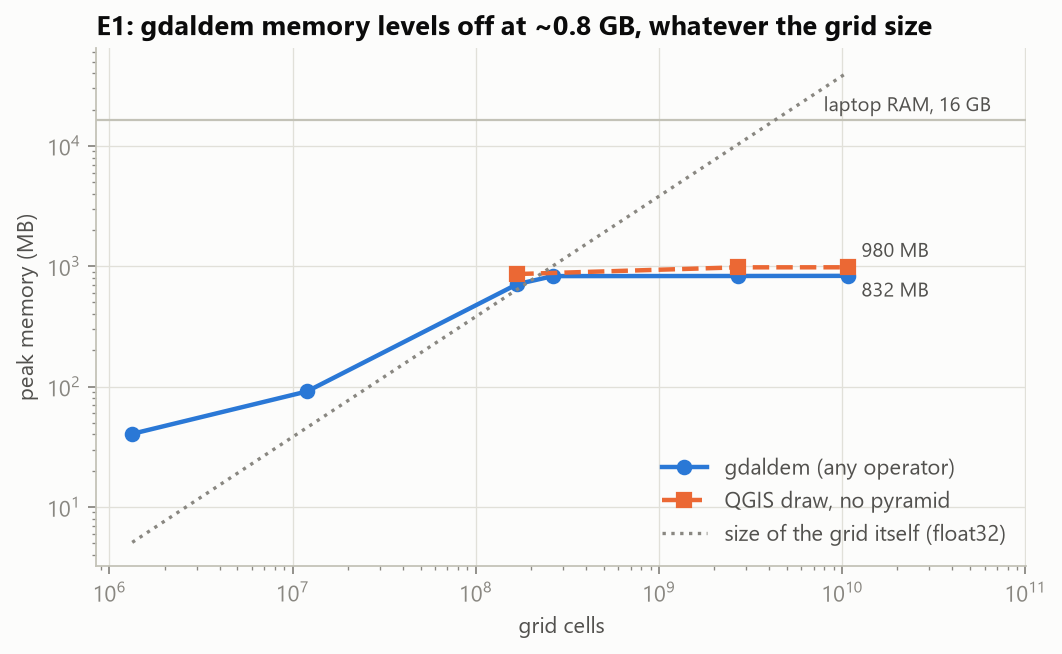
\includegraphics[width=0.49\linewidth]{e1_memory.png}
\caption{Left: run time vs cells. Right: peak memory vs cells.}
\end{figure}
\textbf{Left chart.} Both axes logarithmic; a straight 45$^\circ$ line means ``time proportional to cells''. Slope and
hillshade are straight from 12\,M cells up: \textbf{linear scaling}, about 19--25\,ns per cell. At 90\,m the line bends
because a run lasts 0.07\,s, mostly program start-up. Slope: 4.0\,s (8\,m), 6.6\,s (2\,m real), 54\,s (2\,m synthetic),
208\,s (1\,m).

\textbf{Right chart.} gdaldem's memory \emph{stops growing} at $\sim$0.87\,GB while the grid grows past the 16\,GB line:
gdaldem reads a few rows, computes, writes, moves on (streaming), keeping only GDAL's block cache (5\% of RAM) plus the
program. \textbf{Meaning:} gdaldem cannot ``break'' on memory here. ``Where does it break?'' has the answer ``it doesn't;
it becomes slow''. The real breaking points are memory-hungry approaches (Phase 3's naive version) and display.

\textbf{Cold vs warm} differ by 2\% or less: reading is a small part of the run on this NVMe SSD (cold reads measured at
2.7--3.3\,GB/s), and at 2\,m/1\,m even warm runs read 3.8/14.2\,GB from disk (at 1\,m the file exceeds the cache; at 2\,m
gdaldem's own $\sim$11\,GB output pushes the input out). Our pilot (lit review) saw 3$\times$; it was timed through QGIS on
another laptop, so its first runs most likely included loading the programs.

\begin{figure}[!htbp]
\centering
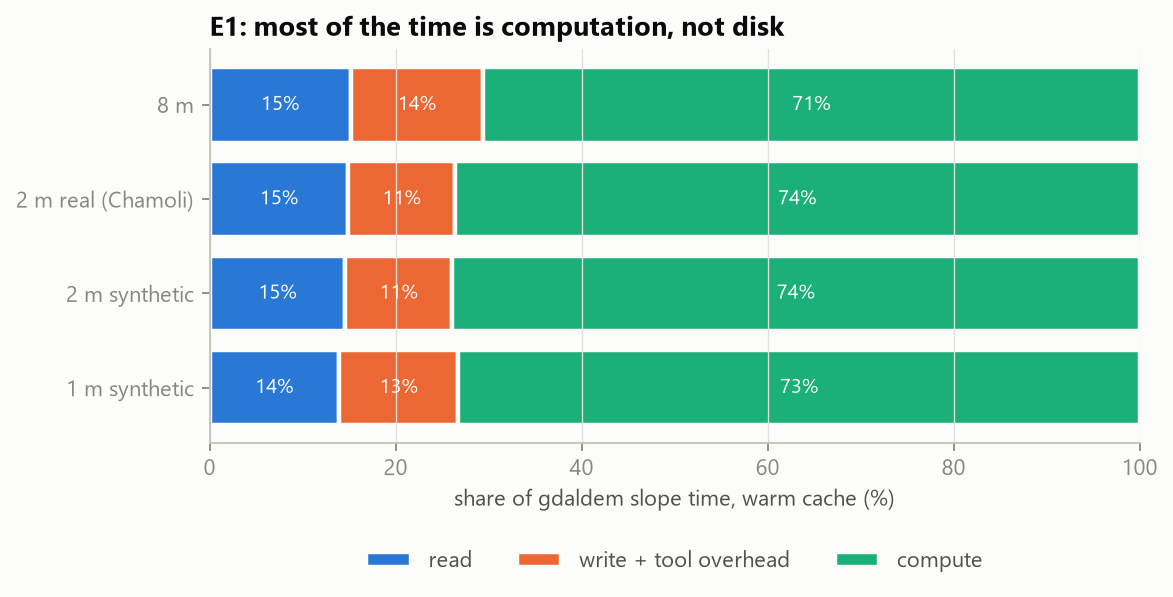
\includegraphics[width=0.49\linewidth]{e1_stages.png}\hfill
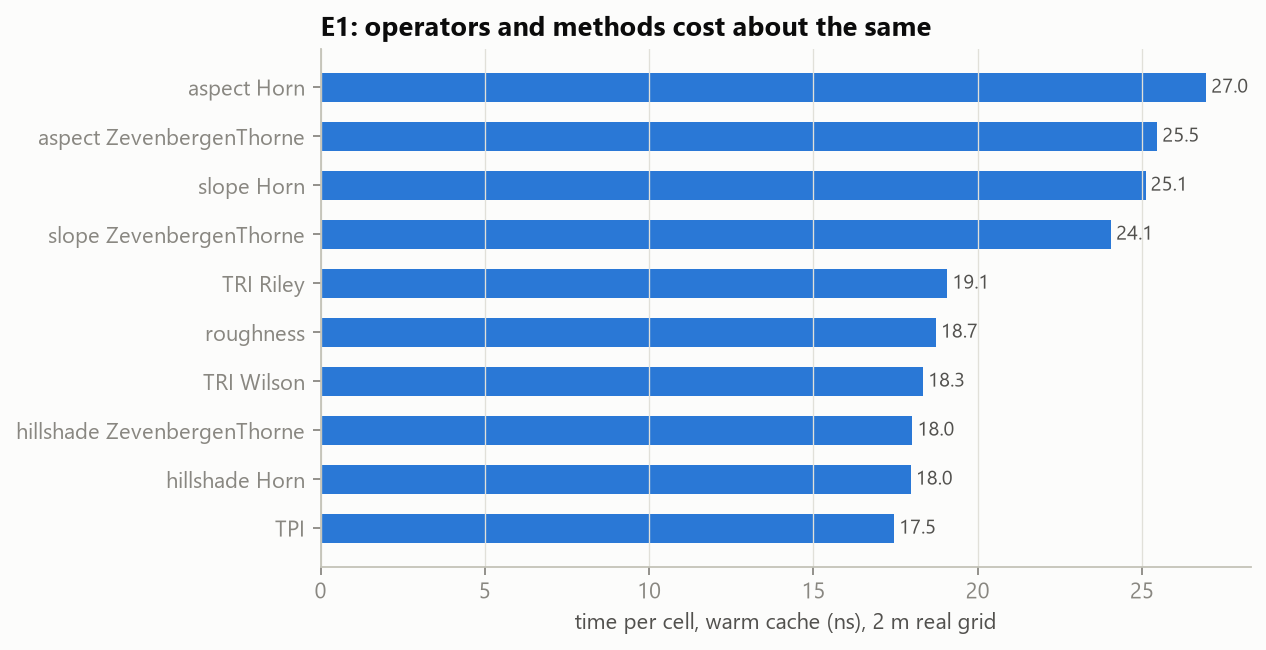
\includegraphics[width=0.49\linewidth]{e1_operators.png}
\caption{Left: stage split of a gdaldem slope run. Right: cost per cell of the ten configurations (2\,m real).}
\end{figure}
\textbf{Stage split.} At every real size $\sim$15\% is reading + decompressing, 11--14\% writing, \textbf{71--74\%
computing}. This contradicts the common claim that data movement dominates: for gdaldem on a fast SSD it is the
arithmetic on one thread. Amdahl: parallelising only the computation gives at most $\sim$3.7$\times$; going further
needs parallel decompression and less writing.

\textbf{Operators.} All ten cost 17.5--27\,ns per cell; Horn vs ZT differ by at most 6\%. The formula is not where
speed comes from; implementation and data movement are. \textbf{Pinning:} on 2\,m synthetic, unpinned cold runs ranged
55.8--108.9\,s (74\% spread); pinned 53.7--55.2\,s (2.8\%).

\subsection{E2: does the file layout matter?}
\begin{figure}[!htbp]
\centering
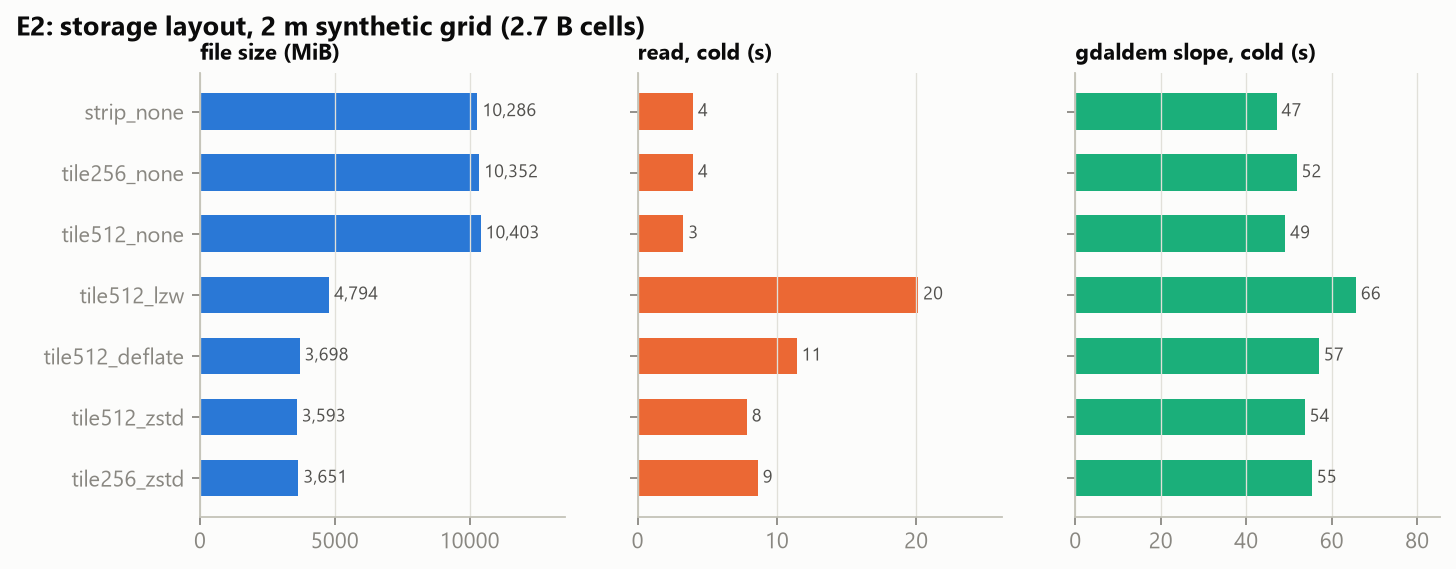
\includegraphics[width=0.85\linewidth]{e2_storage.png}
\caption{File size, read time and gdaldem slope time per storage layout (2\,m synthetic, 2.7\,B cells).}
\end{figure}
\begin{itemize}
  \item \textbf{Size:} uncompressed 10.8--10.9\,GB; LZW 5.0\,GB; DEFLATE 3.9\,GB; ZSTD 3.8\,GB (2.9$\times$ smaller).
  \item \textbf{Read:} uncompressed 3.3--4.0\,s; ZSTD 7.8\,s; DEFLATE 11.4\,s; LZW 20.1\,s (decompression costs CPU).
  \item \textbf{gdaldem slope:} uncompressed strips 47\,s (fastest), ZSTD 54\,s, DEFLATE 57\,s, LZW 66\,s (+39\%), because
  gdaldem decompresses inside its single thread.
  \item \textbf{Write:} compressed files take 6--9$\times$ longer to create (ZSTD 124\,s vs 14\,s): a one-time cost.
  \item \textbf{Tiles vs strips:} strips are fine for a row-by-row pass; tiles matter for reading small windows (the
  viewer); 512 slightly better than 256.
\end{itemize}
\textbf{Meaning:} layout changes gdaldem time by up to $\sim$40\%. Tiled ZSTD (our COGs) is the right compressed format;
avoid LZW.

\subsection{QGIS: why the pyramid matters}
\begin{figure}[!htbp]
\centering
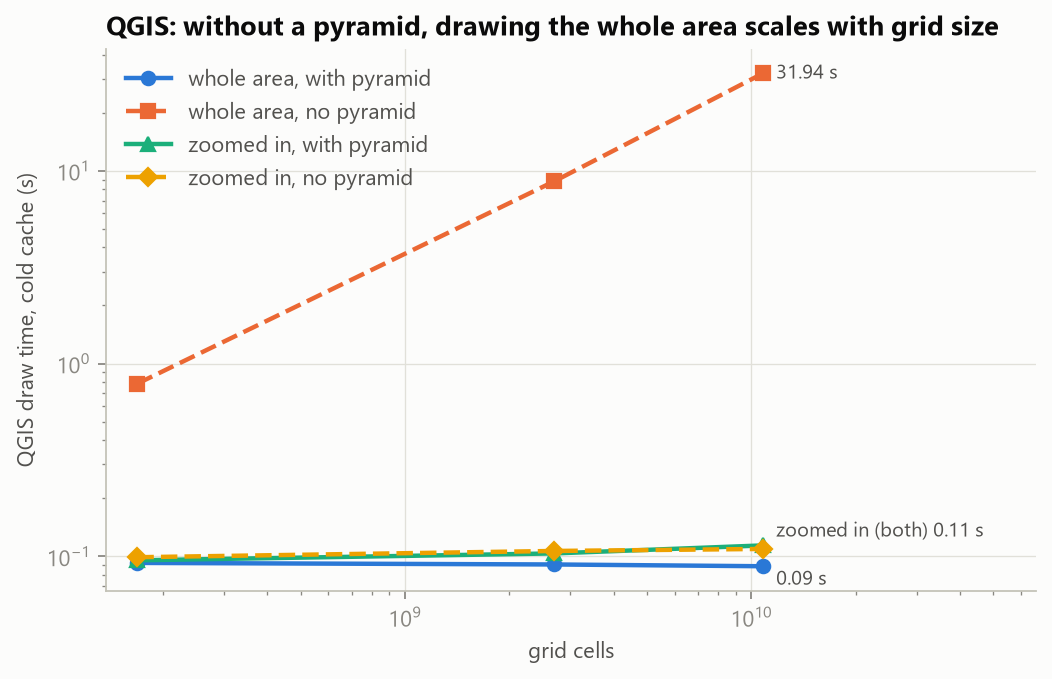
\includegraphics[width=0.58\linewidth]{e1q_render.png}
\caption{QGIS: time to draw one 1920$\times$1080 view.}
\end{figure}
\begin{itemize}
  \item \textbf{Whole area, with pyramid:} 0.09\,s at 8\,m, 2\,m and 1\,m (peak 0.21\,GB): QGIS reads only the level whose
  cells match the screen pixels.
  \item \textbf{Whole area, no pyramid:} 0.79\,s, 8.8\,s, \textbf{31.9\,s} (peak $\sim$1.03\,GB): it decompresses the whole
  full-resolution level (about 12.7\,GB at 1\,m), close to the 29\,s a pure read takes. 360$\times$ slower at 1\,m.
  \item \textbf{Zoomed in:} $\sim$0.1\,s with or without pyramid (only the window is read). \textbf{Opening:} 0.02--0.03\,s.
\end{itemize}
\textbf{Meaning:} the display bottleneck is how much full-resolution data a view must read. A pyramid makes zoomed-out
views cost the same at any grid size, which is the meeting's proposed design.

\key{Phase 2 answer to G1: on this laptop the standard tools do not fail at 1\,m, they stop being practical.
Processing is limited by single-threaded computation; display by reading full-resolution data without a pyramid.}

%=====================================================================
\section{Phase 3 results: our own engine}
\subsection{How the engine works}
\begin{figure}[!htbp]
\centering
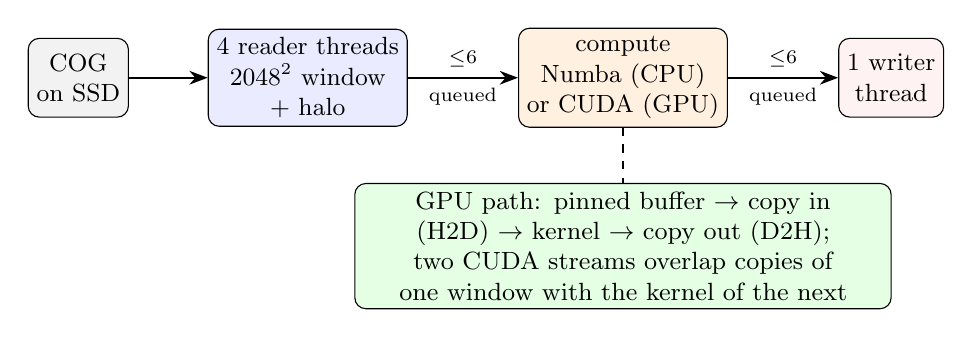
\begin{tikzpicture}[font=\small, node distance=14mm,
  st/.style={draw, rounded corners, align=center, minimum height=10mm, inner sep=3pt},
  arr/.style={-{Stealth}, thick}]
\node[st, fill=gray!10] (cog) {COG\\on SSD};
\node[st, fill=blue!8, right=10mm of cog] (rd) {4 reader threads\\$2048^2$ window\\+ halo};
\node[st, fill=orange!12, right=of rd] (k) {compute\\Numba (CPU)\\or CUDA (GPU)};
\node[st, fill=pink!20, right=of k] (wr) {1 writer\\thread};
\draw[arr] (cog) -- (rd); \draw[arr] (rd) -- node[above,font=\scriptsize]{$\le$6} node[below,font=\scriptsize]{queued} (k);
\draw[arr] (k) -- node[above,font=\scriptsize]{$\le$6} node[below,font=\scriptsize]{queued} (wr);
\node[st, fill=green!10, below=7mm of k, text width=6.6cm] (gpu) {GPU path: pinned buffer $\to$ copy in (H2D) $\to$
kernel $\to$ copy out (D2H); two CUDA streams overlap copies of one window with the kernel of the next};
\draw[dashed] (k) -- (gpu);
\end{tikzpicture}
\caption{The engine: a bounded three-stage pipeline. Memory stays flat whatever the grid size.}
\end{figure}
\code{demlab/engine.py} (pipeline), \code{demlab/kernels/numba\_k.py} (CPU), \code{demlab/kernels/cuda\_k.py} and
\code{demlab/gpu.py} (GPU), \code{demlab/cli.py} (command line used by the benchmarks). All ten \code{gdaldem}
configurations; slope, aspect and hillshade fused.

\subsection{Correctness}
119 unit tests and a full-grid check: CPU and GPU engines vs \code{gdaldem} on \textbf{every cell} of the whole 90\,m,
30\,m, 8\,m and 2\,m grids, all 10 configurations (1.3\,M to 247\,M valid cells per grid). Nodata masks identical and all
values within tolerance. The only exception: our float64 CPU engine differs in Horn aspect on nearly flat cells (up to
0.08\% of cells) and Horn slope on one cell (0.022$^\circ$), because \code{gdaldem} adds the Horn neighbours in float32.
With that rounding reproduced, every cell of all four grids matches; the float32 GPU kernel matches with no exception.

\subsection{E3: CPU engine vs gdaldem}
\begin{table}[!htbp]
\centering\small
\caption{Slope (Horn), warm cache. ``Same cores'' = the 12 performance-core threads gdaldem used.}
\begin{tabularx}{\linewidth}{lrRRRRR}
\toprule
Grid & Cells & gdaldem & Engine, same cores & Speed-up & Engine, 22 thr. & Peak memory \\
\midrule
8\,m & 169\,M & 4.02\,s & 1.94\,s & 2.1$\times$ & 2.28\,s & 1.35\,GB \\
2\,m real & 264\,M & 6.63\,s & 2.53\,s & 2.6$\times$ & 2.72\,s & 1.37\,GB \\
2\,m synthetic & 2.7\,B & 53.7\,s & 16.3\,s & 3.3$\times$ & 16.4\,s & 1.42\,GB \\
1\,m synthetic & 10.8\,B & 208.4\,s & \textbf{60.3\,s} & \textbf{3.5$\times$} & 68.2\,s & 1.43\,GB \\
\bottomrule
\end{tabularx}
\end{table}
\begin{figure}[!htbp]
\centering
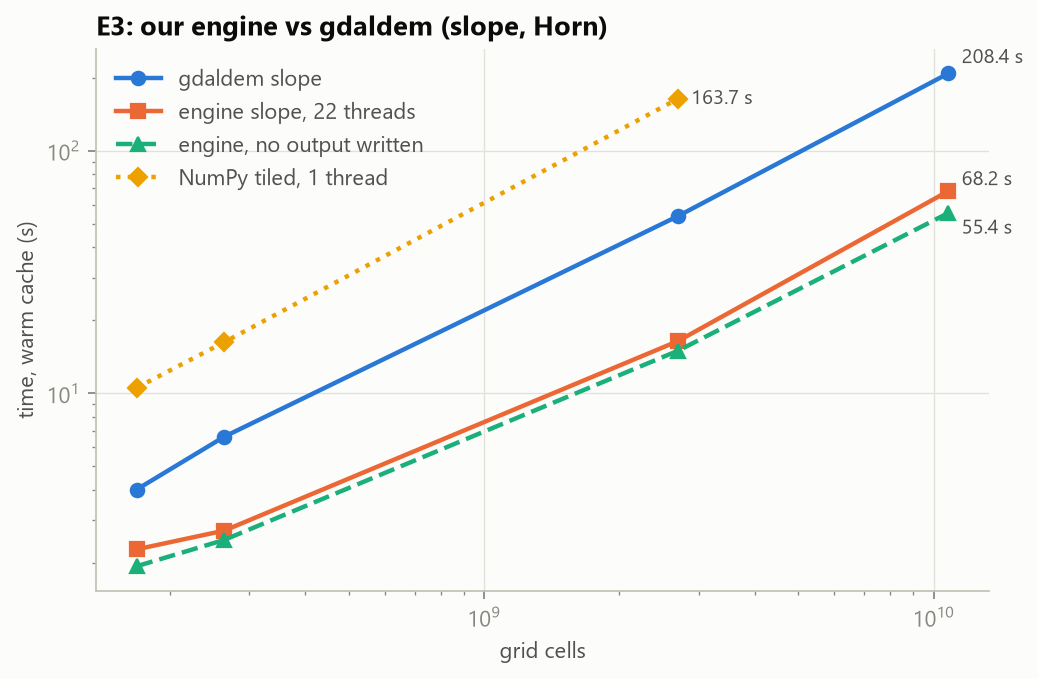
\includegraphics[width=0.49\linewidth]{e3_scaling.png}\hfill
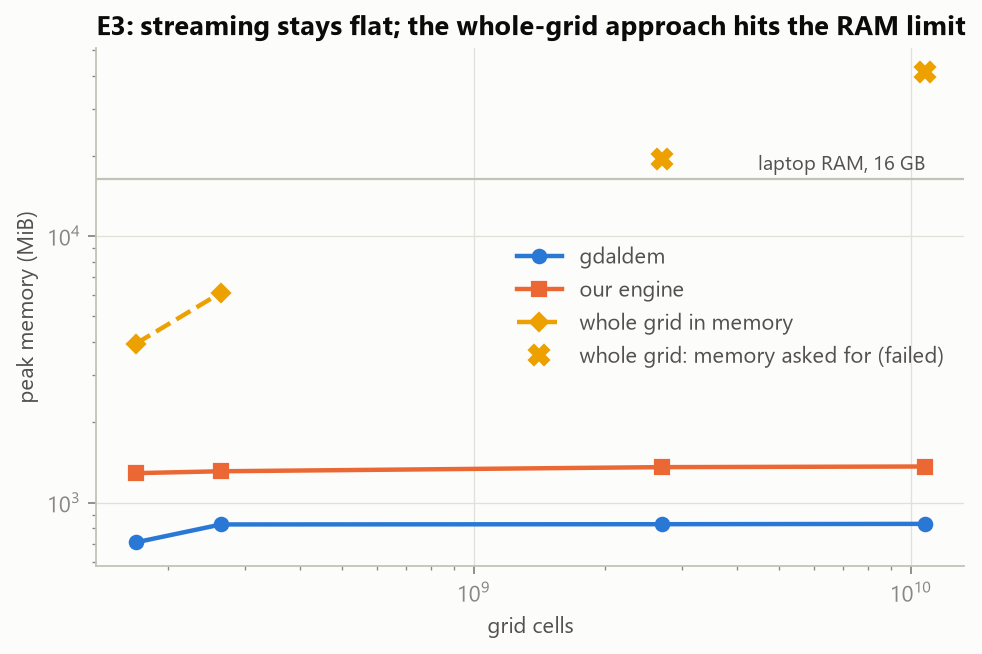
\includegraphics[width=0.49\linewidth]{e3_memory.png}
\caption{Left: engine vs gdaldem. Right: memory: the engine is flat; the naive whole-grid version fails.}
\end{figure}
\begin{itemize}
  \item \textbf{2.1--3.5$\times$ faster on the same cores, growing with size} (1\,m: 5.6 vs 19\,ns per cell). Small grids gain
  less because $\sim$1\,s of every run is fixed cost (Python start-up 0.5--0.6\,s, loading the compiled kernel 0.45\,s).
  \item \textbf{12 P-core threads beat all 22} (1\,m: 60\,s vs 68\,s): slow cores hold the evenly split work up.
  \item \textbf{Memory flat} at $\sim$1.4\,GB (gdaldem 0.87\,GB).
  \item \textbf{Breaking point of the naive approach:} $\sim$24 bytes per cell (4.1\,GB at 8\,m, 6.4\,GB at 2\,m real). At 2\,m
  synthetic it held 9.6\,GB when a further 10.7\,GB allocation was refused (whole run would need $\sim$65\,GB); at 1\,m the
  first allocation (43\,GB) was refused. Whole-grid processing stops at roughly 0.5--0.7\,B cells on 16\,GB.
  \item \textbf{Speed comes from the compiled parallel kernel}: the same pipeline with a single-threaded NumPy kernel is
  2.6--3$\times$ \emph{slower} than gdaldem.
  \item \textbf{Every operator faster}: all 10 configurations 1.3--2.0$\times$ at 8\,m, 1.7--2.6$\times$ at 2\,m real.
  \item \textbf{Three products in one pass}: 3.3\,s vs 11.3\,s for three gdaldem runs at 8\,m (3.4$\times$), 4.4\,s vs 18.5\,s at
  2\,m real (4.2$\times$); 135\,s at 1\,m.
\end{itemize}
\begin{figure}[!htbp]
\centering
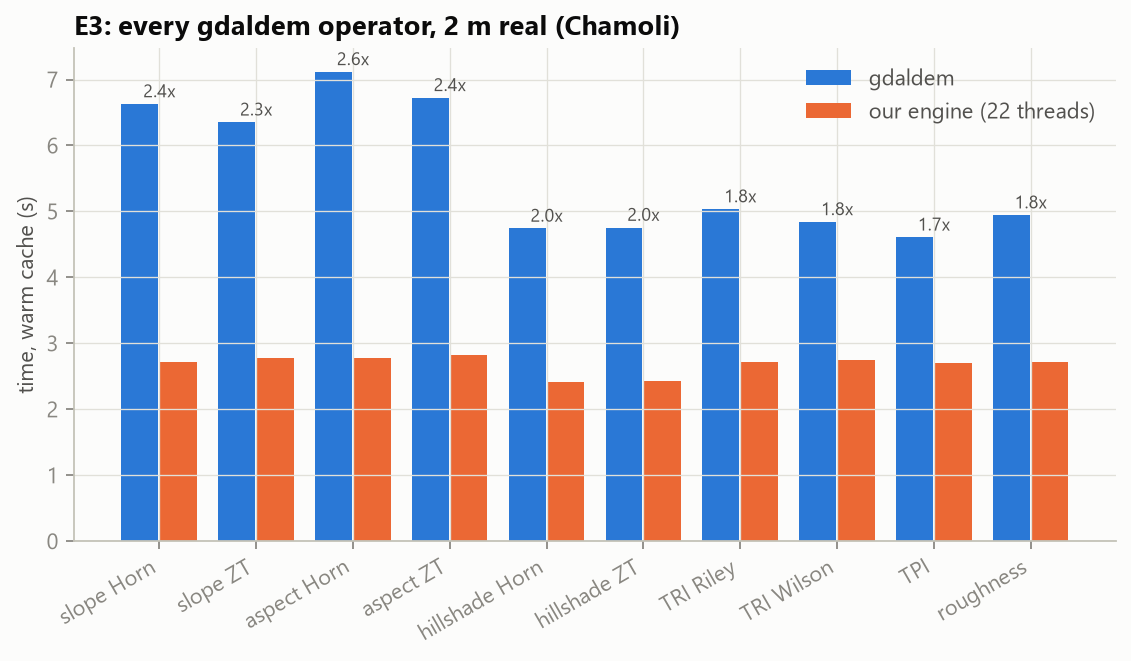
\includegraphics[width=0.49\linewidth]{e3_operators.png}\hfill
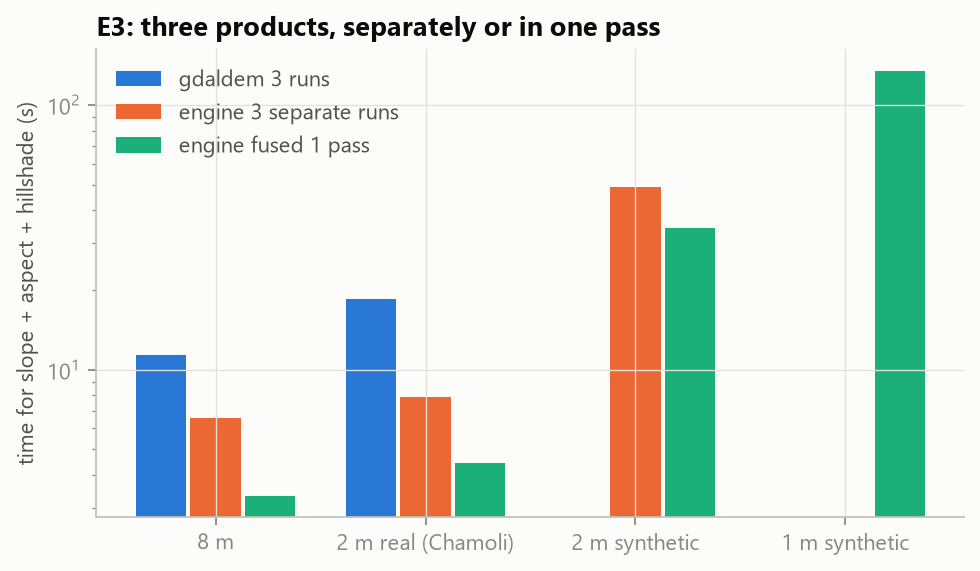
\includegraphics[width=0.49\linewidth]{e3_products.png}
\caption{Left: all ten configurations (2\,m real). Right: three products separately or fused.}
\end{figure}

\textbf{Where the time goes} (slope, 22 threads, warm, 1\,m): total 68.2\,s; kernel 33\,s; the single writer thread is busy
65\,s writing 43\,GB ($\sim$0.66\,GB/s): \textbf{write-bound}. Without writing (55.4\,s) it is \textbf{read-bound}: 23\,s
waiting for windows to be decompressed. Compressed output (ZSTD) is 40\% smaller but slower (21.2 vs 16.4\,s at 2\,m
synthetic). Cold vs warm: almost no difference.

\begin{figure}[!htbp]
\centering
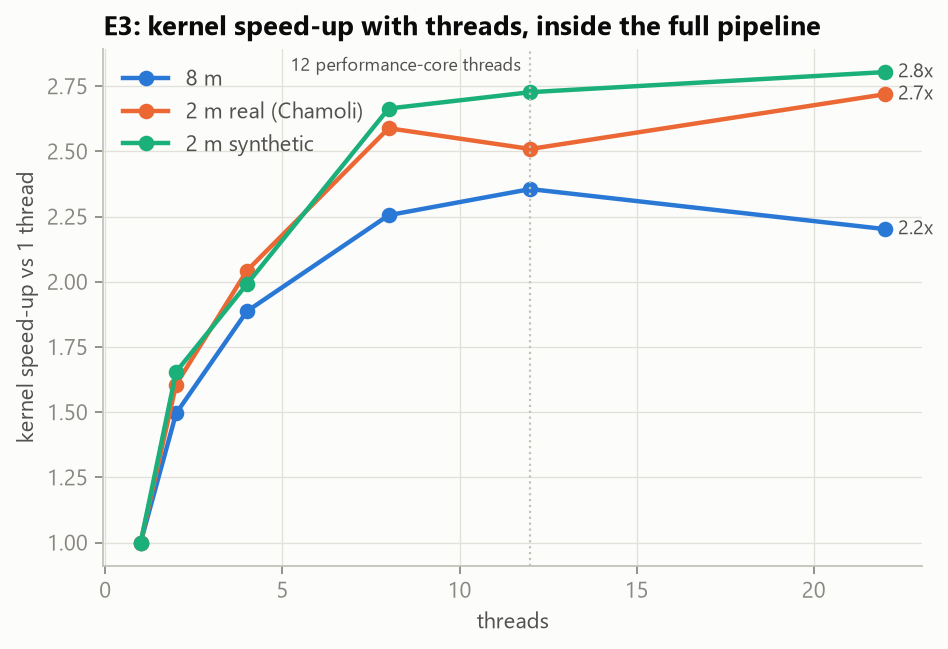
\includegraphics[width=0.45\linewidth]{e3_threads.png}\hfill
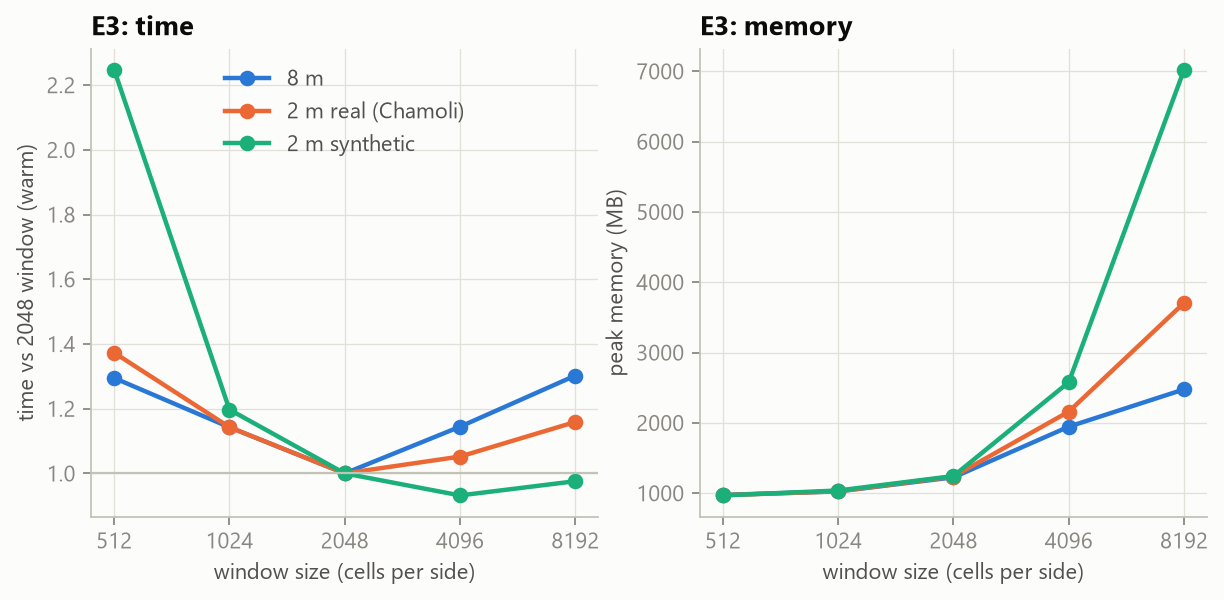
\includegraphics[width=0.53\linewidth]{e3_window.png}
\caption{Left: kernel speed-up with threads inside the pipeline. Right: window size.}
\end{figure}
\textbf{Threads:} inside the pipeline the kernel speeds up only 2.2--2.8$\times$ from 1 to 22 threads; alone in memory it
scales to $\sim$16 threads (9.5 $\to$ 1.7\,ns per cell). It shares cores with decompression and writing.
\textbf{Window size:} 2048 is best. Small windows are slow because of the halo: the one-cell border forces the
neighbouring compressed 512-tiles to be decoded again, $(w/512+2)^2$ instead of $(w/512)^2$ tiles: 9$\times$ extra work at
512, 2.25$\times$ at 2048. An 8192 window holds 7.4\,GB in flight for no gain.

\subsection{E4: the GPU engine}
\begin{table}[!htbp]
\centering\small
\caption{Slope (Horn), warm: gdaldem, CPU engine (12 threads), GPU engine.}
\begin{tabularx}{\linewidth}{lRRRRRR}
\toprule
Grid & gdaldem & CPU engine & GPU engine & GPU vs CPU & GPU vs gdaldem & GPU, no output \\
\midrule
8\,m & 4.02\,s & 1.94\,s & 1.90\,s & 1.0$\times$ & 2.1$\times$ & 1.80\,s \\
2\,m real & 6.63\,s & 2.53\,s & 2.18\,s & 1.2$\times$ & 3.0$\times$ & 2.03\,s \\
2\,m synthetic & 53.7\,s & 16.3\,s & 11.3\,s & 1.4$\times$ & 4.7$\times$ & 9.3\,s \\
1\,m synthetic & 208.4\,s & 60.3\,s & \textbf{43.8\,s} & 1.4$\times$ & \textbf{4.75$\times$} & 33.9\,s \\
\bottomrule
\end{tabularx}
\end{table}
\begin{figure}[!htbp]
\centering
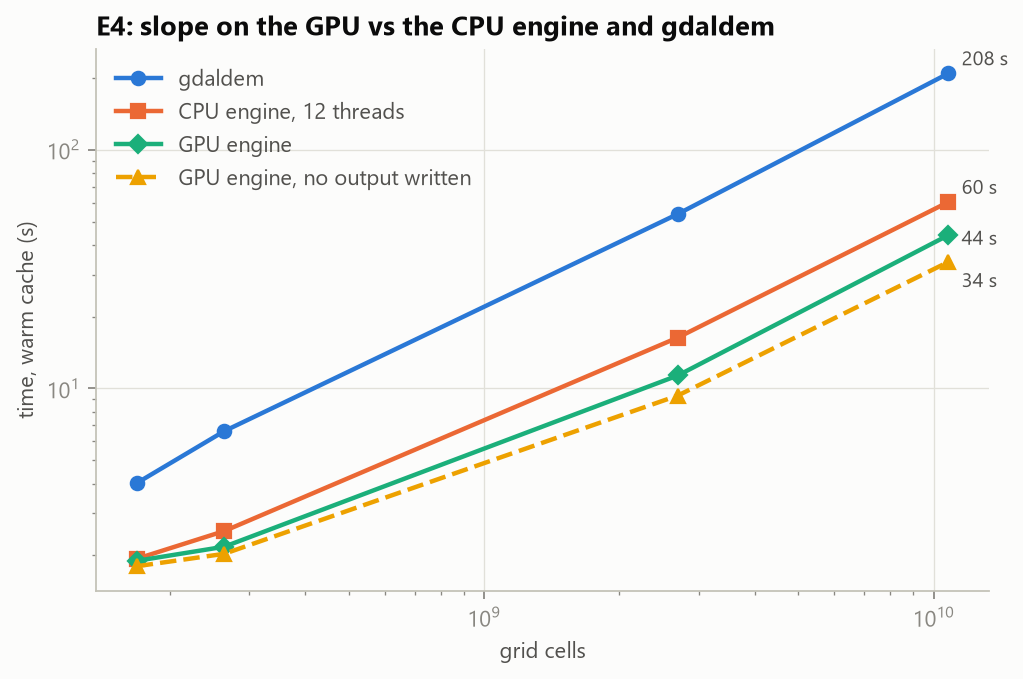
\includegraphics[width=0.49\linewidth]{e4_scaling.png}\hfill
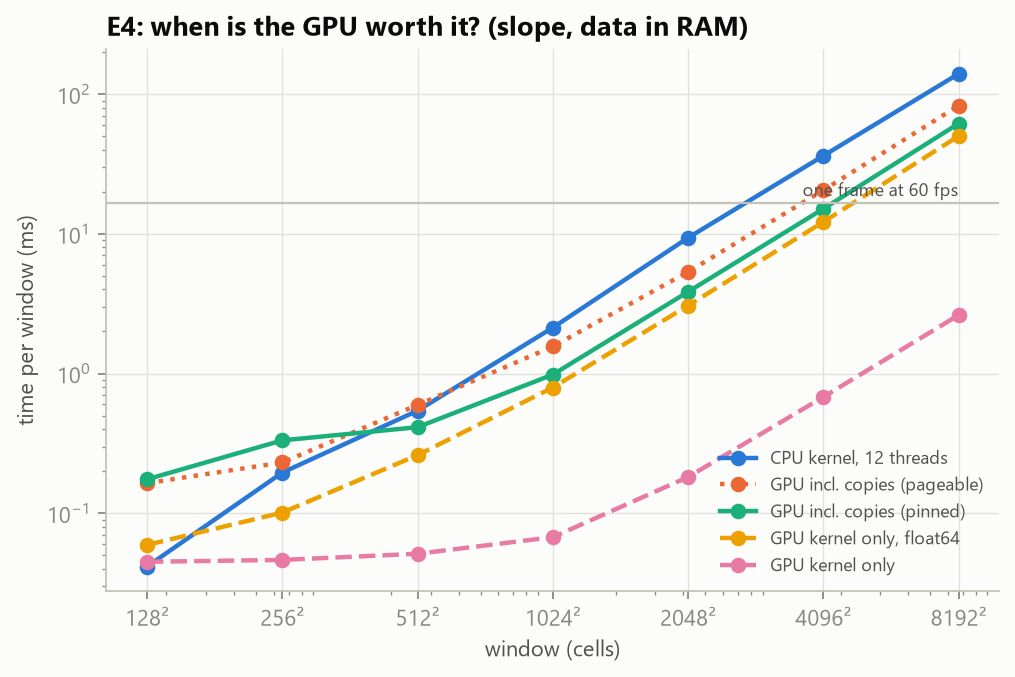
\includegraphics[width=0.49\linewidth]{e4_crossover.png}
\caption{Left: GPU vs CPU vs gdaldem. Right: one window in memory: kernel alone vs kernel with copies vs CPU.}
\end{figure}
\begin{itemize}
  \item \textbf{Kernel 50$\times$ faster, run 1.0--1.4$\times$ faster.} The GPU kernel needs 1.1\,s for the whole 1\,m grid
  (CPU engine's kernel: 34\,s).
  \item \textbf{Copying is 95\% of the GPU's time}: for a $2048^2$ window, kernel 0.18\,ms, kernel + copies 3.85\,ms.
  \item \textbf{Crossover:} the GPU (with copies) beats the CPU from $512^2$ cells for slope ($256^2$ for three products);
  below that a round trip ($\geq$0.17\,ms) loses. From $1024^2$ up: 2.2--2.4$\times$ (slope), 3.6--3.7$\times$ (3 products).
  \item \textbf{Fused products gain the most}: 81\,s at 1\,m vs 135\,s CPU (1.7$\times$); 3.1\,s vs 18.5\,s for three gdaldem runs
  on 2\,m real (5.9$\times$).
  \item \textbf{How the GPU is used matters more than the GPU} (2\,m synthetic): straightforward CuPy port 17.0\,s
  (\emph{slower} than the CPU engine, 16.3\,s) $\to$ own kernel 12.6\,s $\to$ pinned buffers 11.1\,s $\to$ 2 streams 11.3\,s.
  The GPU part halves at each step (14.5 $\to$ 7.6 $\to$ 3.7 $\to$ 2.0\,s) but the total stops improving.
  \item \textbf{float64} makes the kernel 8--24$\times$ slower but the total almost unchanged (11.5 vs 11.3\,s).
  \item \textbf{GPU memory never the limit}: at most 2.0\,GiB window by window; a whole grid at once would need 22\,GB (2\,m
  synthetic) or 86\,GB (1\,m).
\end{itemize}
\begin{figure}[!htbp]
\centering
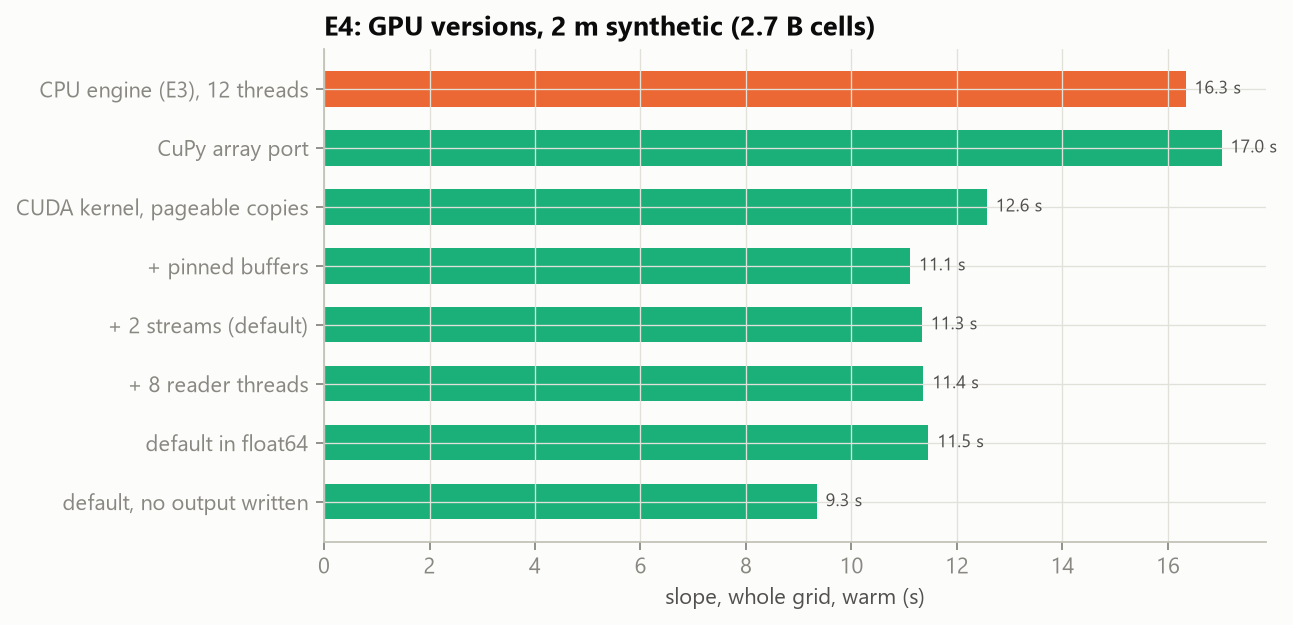
\includegraphics[width=0.5\linewidth]{e4_ladder.png}\hfill
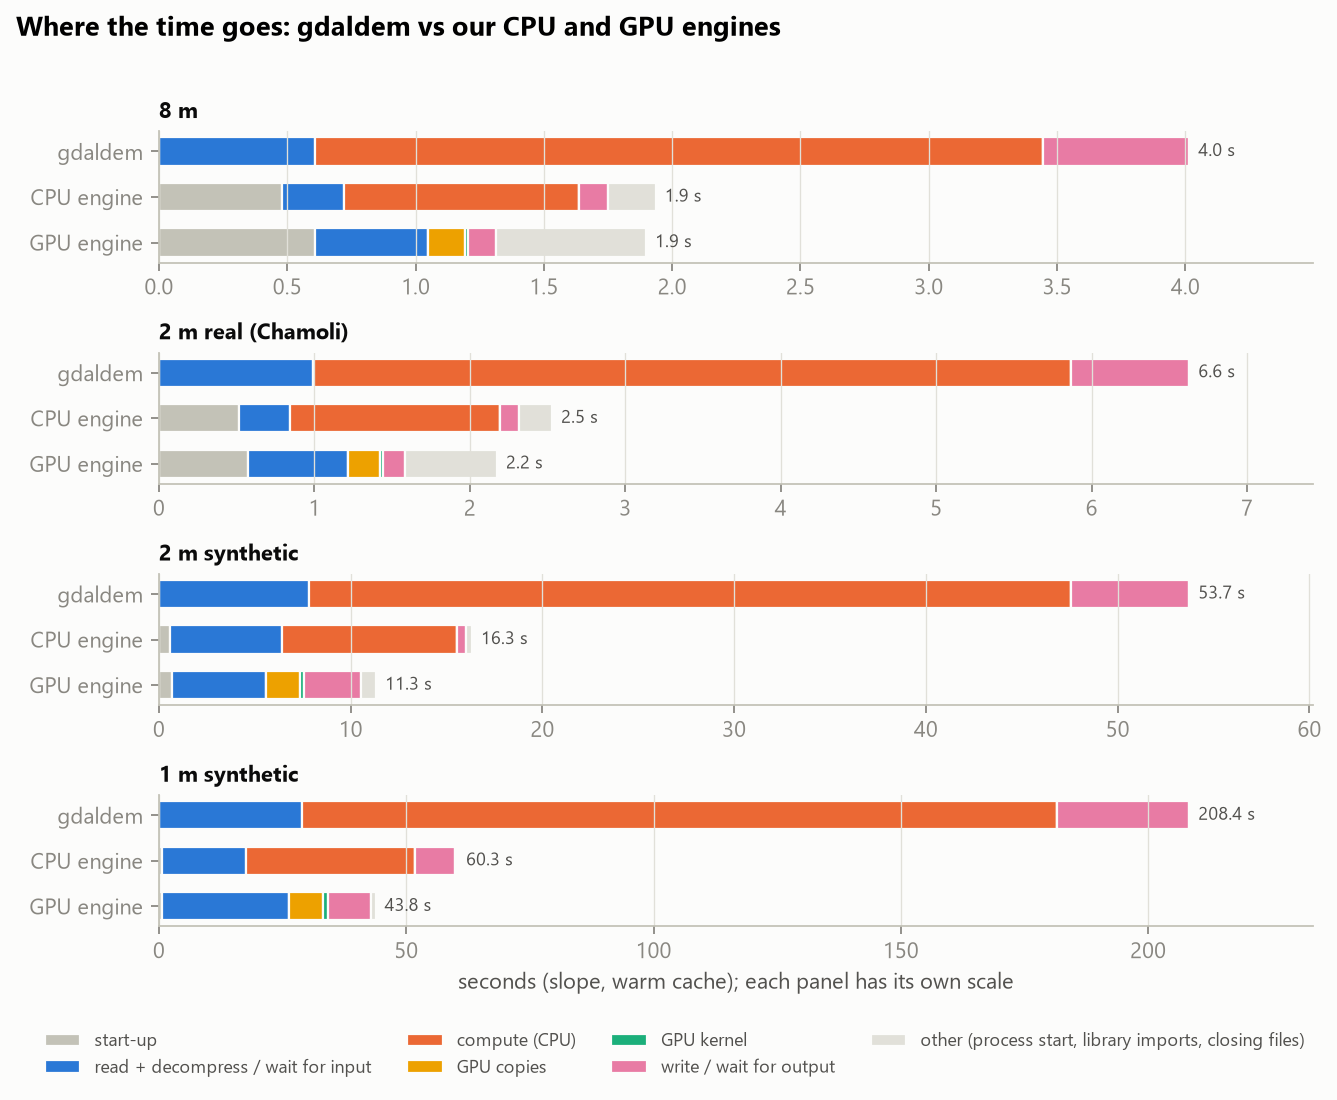
\includegraphics[width=0.48\linewidth]{e4_stages.png}
\caption{Left: GPU optimisation steps (2\,m synthetic). Right: where the time goes, gdaldem vs CPU vs GPU engine.}
\end{figure}
\textbf{The bottleneck moves:} at 1\,m the GPU engine waits 25.7\,s for input and spends 7.8\,s on the GPU. With 8 readers
the read wait falls to 3.2\,s, but then the writer is the limit (30.6\,s wait, 43\,GB at $\sim$1.1\,GB/s): total only 43.8
$\to$ 42.6\,s. Computation $\to$ decompression $\to$ writing.

\key{Phase 3 answer: parallel computation removes gdaldem's bottleneck (2--3.5$\times$, up to 4.75$\times$ with the GPU), and
the run becomes limited by moving data: decompressing input, copying over PCIe, writing output. Faster kernels alone
cannot help any more; reading and writing less can, which is exactly what on-demand display does.}

%=====================================================================
\section{Phase 4 results: derivatives on demand from the pyramid (G2)}
\subsection{Accuracy}
\begin{table}[!htbp]
\centering\small
\caption{Slope from each pyramid level vs the full-resolution truth (fully valid cells).}
\begin{tabularx}{\linewidth}{llRRRRRR}
\toprule
DEM & Level & Cells scored & RMSE & Bias & $>$5$^\circ$ & Shown / true mean & RMSE exact pyramid \\
\midrule
Chamoli 2\,m & 4\,m & 61.4\,M & \textbf{2.3$^\circ$} & $-$0.5$^\circ$ & 4.1\% & 0.99 & 2.3$^\circ$ \\
 & 8\,m & 15.2\,M & \textbf{4.4$^\circ$} & $-$1.2$^\circ$ & 15.5\% & 0.97 & 4.4$^\circ$ \\
 & 16\,m & 3.7\,M & \textbf{5.6$^\circ$} & $-$2.2$^\circ$ & 23.4\% & 0.94 & 5.6$^\circ$ \\
 & 32\,m & 0.91\,M & \textbf{6.4$^\circ$} & $-$3.3$^\circ$ & 30.5\% & 0.91 & 6.4$^\circ$ \\
 & 64\,m & 0.22\,M & \textbf{7.9$^\circ$} & $-$5.0$^\circ$ & 43.1\% & 0.87 & 7.8$^\circ$ \\
 & 128\,m & 51\,k & \textbf{10.0$^\circ$} & $-$7.3$^\circ$ & 57.8\% & 0.81 & 9.9$^\circ$ \\
\midrule
HMA 8\,m & 16\,m & 29.6\,M & \textbf{2.6$^\circ$} & $-$0.7$^\circ$ & 6.6\% & 0.98 & 2.4$^\circ$ \\
 & 32\,m & 6.5\,M & \textbf{4.0$^\circ$} & $-$1.6$^\circ$ & 15.6\% & 0.95 & 3.9$^\circ$ \\
 & 64\,m & 1.3\,M & \textbf{5.3$^\circ$} & $-$2.9$^\circ$ & 26.3\% & 0.90 & 5.3$^\circ$ \\
 & 128\,m & 0.23\,M & \textbf{6.9$^\circ$} & $-$4.5$^\circ$ & 40.5\% & 0.83 & 6.9$^\circ$ \\
 & 256\,m & 29\,k & \textbf{9.0$^\circ$} & $-$6.8$^\circ$ & 58.7\% & 0.73 & 8.8$^\circ$ \\
\bottomrule
\end{tabularx}
\end{table}
\begin{figure}[!htbp]
\centering
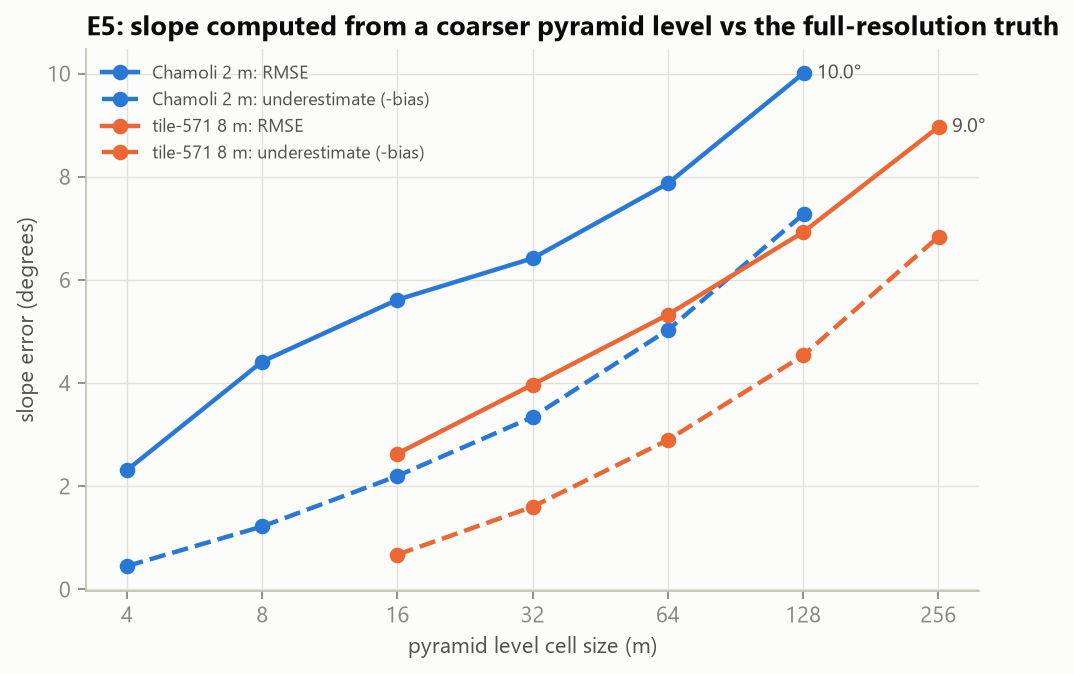
\includegraphics[width=0.49\linewidth]{e5_error_by_level.png}\hfill
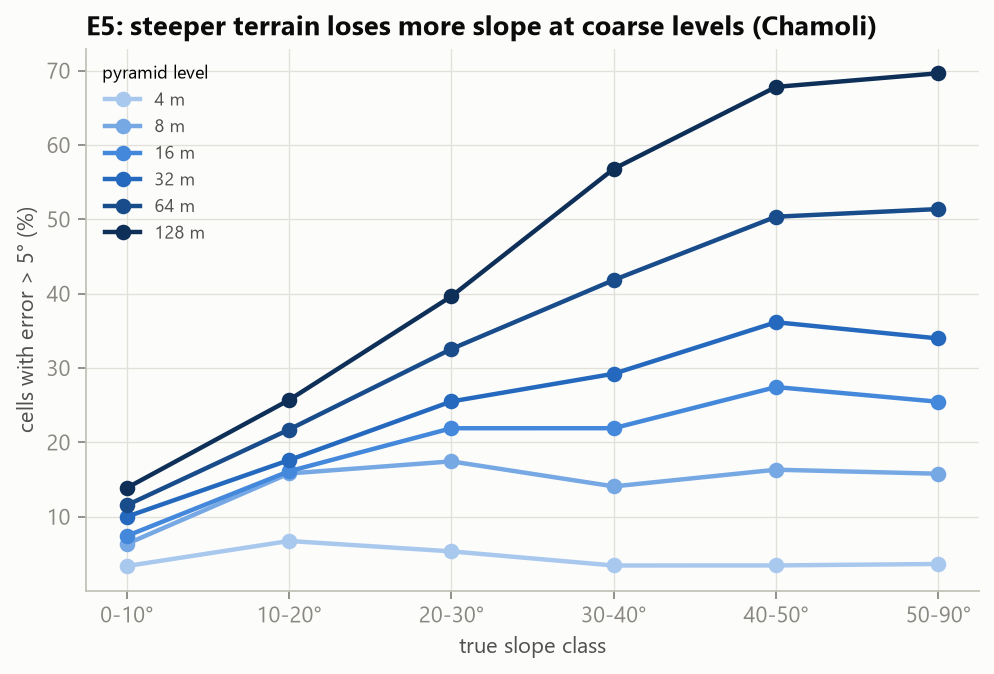
\includegraphics[width=0.49\linewidth]{e5_by_class.png}
\caption{Left: RMSE and underestimate per level. Right: share of cells off by $>$5$^\circ$ by true slope class (Chamoli).}
\end{figure}
\begin{figure}[!htbp]
\centering
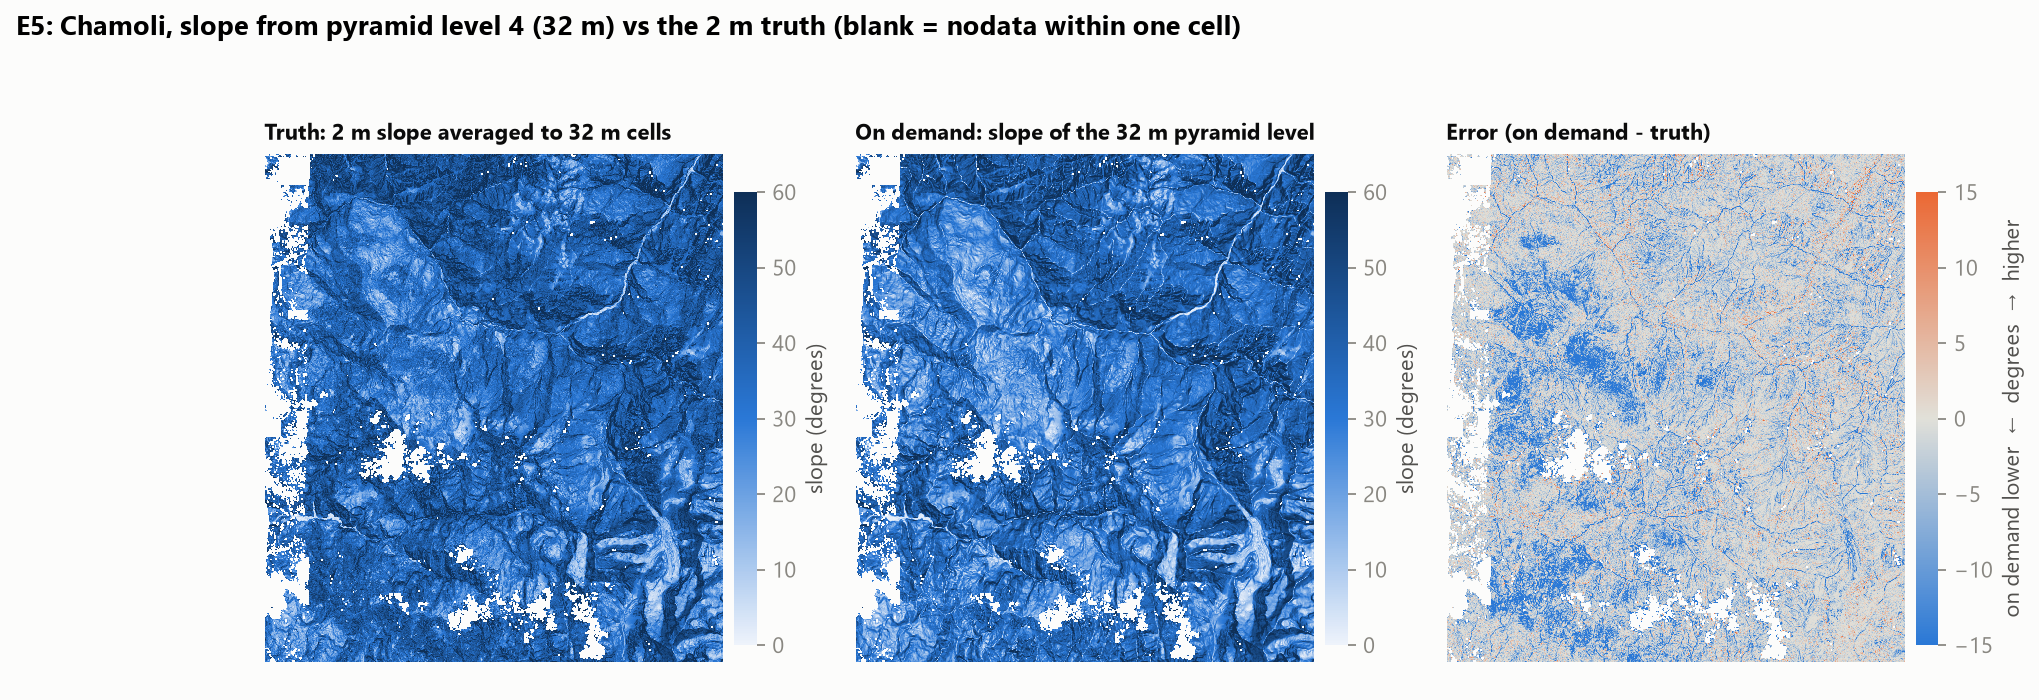
\includegraphics[width=\linewidth]{e5_maps.png}
\caption{Chamoli at 32\,m: truth, on demand, error (blue = on demand lower).}
\end{figure}
\begin{itemize}
  \item \textbf{Why too low:} averaging the DEM smooths the terrain before slope is computed, which removes steepness.
  Known since Zhang \& Montgomery (1994) for coarser grids; new here is the measurement on pyramid levels against the
  time saved.
  \item \textbf{Levels up, not metres:} both DEMs give similar errors for the same number of levels up. Rule of thumb:
  $\sim$2.5$^\circ$ RMSE one level up, then on average $\sim$1.5$^\circ$ more per further level.
  \item \textbf{Steep ground loses most:} at 32\,m the bias is $-$0.9$^\circ$ on 0--10$^\circ$ ground, $-$4.0$^\circ$ on
  40--50$^\circ$. The share of terrain $\geq$45$^\circ$ falls from 29.3\% (truth) to 21.9\% at 32\,m and from 27.4\% to 10.1\% at
  128\,m: thresholded maps (landslide susceptibility) must not use coarse levels.
  \item \textbf{Aspect survives:} median error 1.8$^\circ$ (4\,m) to 8.5$^\circ$ (128\,m); only 1.4--13.7\% of cells off by more
  than 22.5$^\circ$ (one 16-point compass sector).
  \item \textbf{Pyramid of good data beats another sensor:} 2\,m averaged to 8\,m: 4.5$^\circ$ vs HMA 8\,m 8.6$^\circ$; to 30\,m:
  6.3$^\circ$ vs Copernicus 30\,m 9.4$^\circ$; to 90\,m: 8.7$^\circ$ vs 9.9$^\circ$.
  \item \textbf{GDAL's overviews behave like an exact pyramid} (within 0.2$^\circ$) despite the rounding.
\end{itemize}
\begin{figure}[!htbp]
\centering
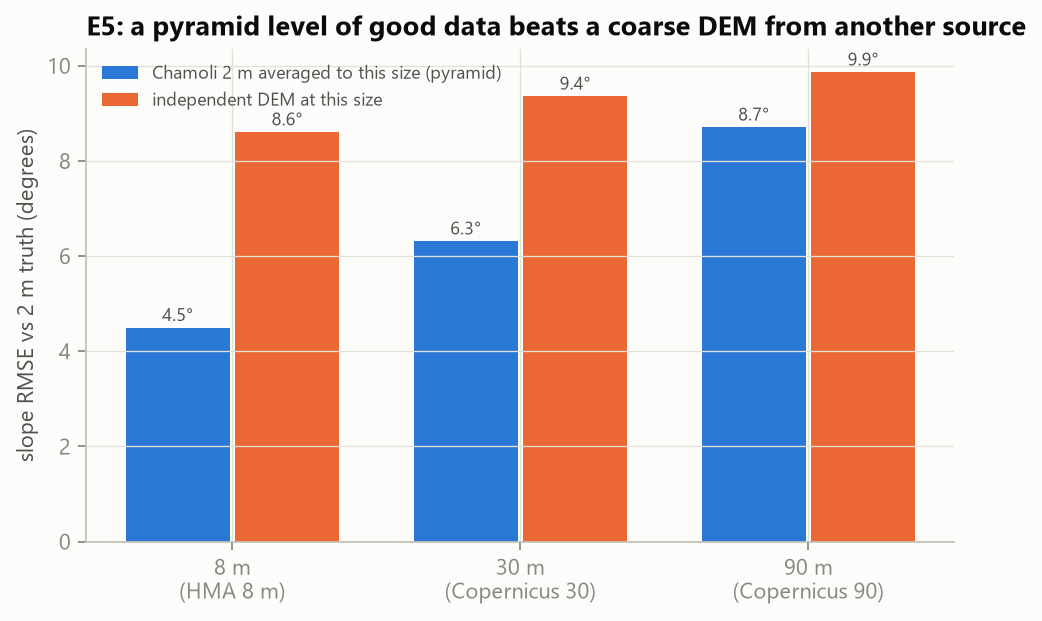
\includegraphics[width=0.55\linewidth]{e5_sensors.png}
\caption{A pyramid level of the 2\,m data vs an independent DEM of the same resolution.}
\end{figure}

\subsection{Time}
\begin{table}[!htbp]
\centering\small
\caption{One $512^2$ display tile, median of 8 places (ms, warm / cold), and time saved by on demand (warm).}
\begin{tabularx}{\linewidth}{llRRRR}
\toprule
DEM & Level & On demand & Full res + average & Precomputed & Time saved \\
\midrule
Chamoli & 4\,m & 7.2 / 7.6 & 56 / 55 & 5.0 / 6.1 & 7.8$\times$ \\
 & 8\,m & 6.4 / 7.3 & 192 / 194 & 4.3 / 5.3 & 30$\times$ \\
 & 16\,m & 6.6 / 7.3 & 624 / 626 & 3.8 / 4.9 & 94$\times$ \\
 & 32\,m & 6.4 / 6.8 & 2867 / 2823 & 3.8 / 4.8 & \textbf{447$\times$} \\
\midrule
HMA 8\,m & 16\,m & 6.9 / 7.1 & 52 / 57 & 4.2 / 5.3 & 7.6$\times$ \\
 & 128\,m & 6.2 / 7.0 & 1186 / 1204 & 3.2 / 4.1 & 193$\times$ \\
\bottomrule
\end{tabularx}
\end{table}
\begin{figure}[!htbp]
\centering
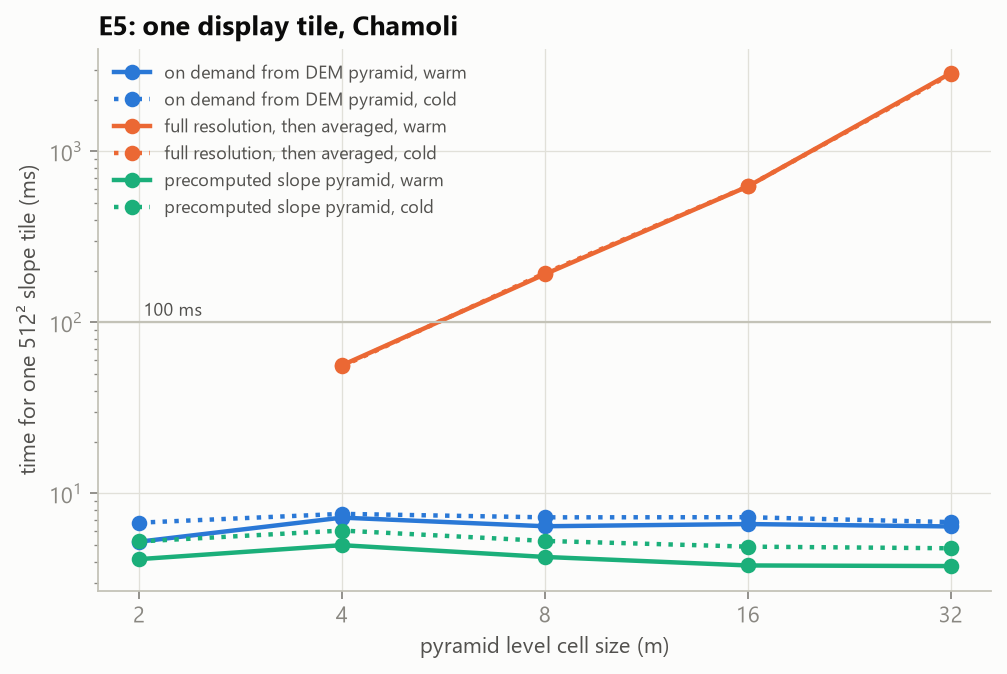
\includegraphics[width=0.49\linewidth]{e5_tile_time.png}\hfill
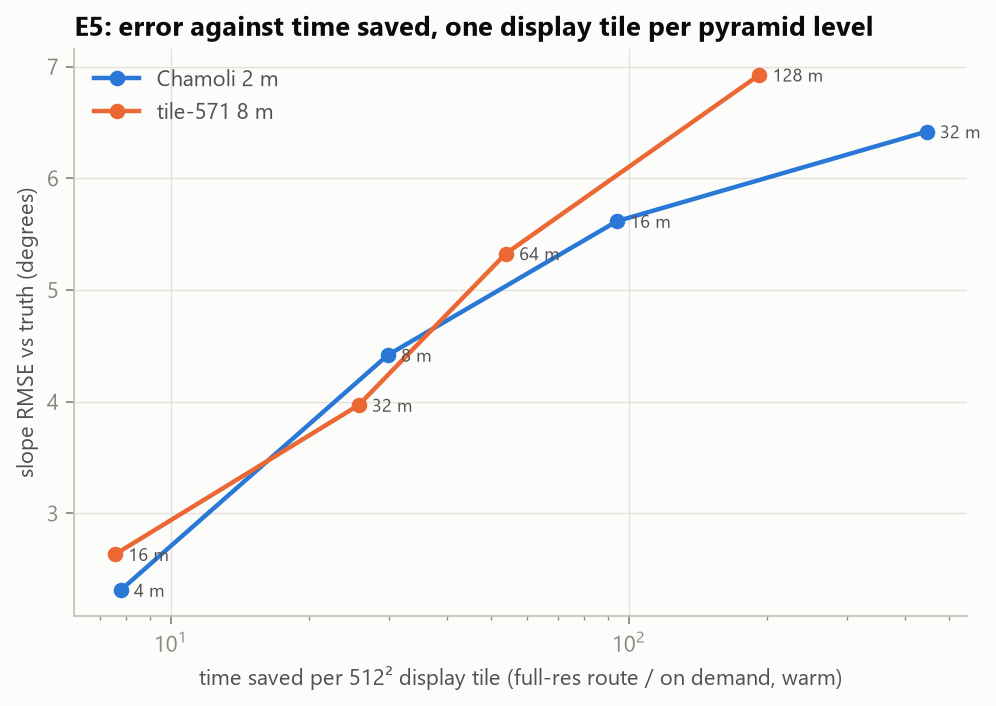
\includegraphics[width=0.49\linewidth]{e5_tradeoff.png}
\caption{Left: tile time per level, three routes. Right: the G2 trade-off, RMSE vs time saved.}
\end{figure}
\begin{itemize}
  \item \textbf{On demand is flat} (5--8\,ms per tile at every level): a tile always reads $514^2$ cells. The exact route reads
  4$\times$ more ground per level (2.9\,s per tile at 32\,m). Whole Chamoli area at 32\,m: 13\,ms vs 4.7\,s.
  \item \textbf{Precomputed} is 1--3\,ms faster per tile and exact, but costs a full pass and storage per derivative: Chamoli
  slope pyramid 10.6\,s and 1.0\,GB (more than the 650\,MB DEM pyramid); all ten configurations $\sim$10\,GB, rebuilt for every
  parameter change. On demand needs none.
  \item Cold vs warm: at most 1.5\,ms per tile (on demand).
\end{itemize}

\key{Phase 4 answer to G2: each pyramid level up saves 2--5$\times$ time per view (8--450$\times$ per tile for 1--4 levels) and
costs $\sim$2.5$^\circ$ slope RMSE for the first level and $\sim$1.5$^\circ$ per further level, as a systematic
underestimate, worst on steep ground. Aspect costs much less. Good for display; not for slope thresholds.}

%=====================================================================
\section{The whole story (what to say in the presentation)}
\begin{enumerate}
  \item \textbf{Problem:} a 1\,m DEM of our area is 43\,GB, 2.6$\times$ the laptop's RAM.
  \item \textbf{Standard tools} (gdaldem, QGIS) don't crash: they stream. But slope takes 3.5\,min on one thread, and
  displaying without a pyramid takes 32\,s per redraw. Bottleneck: single-threaded computation; for display, reading.
  \item \textbf{Our engine} uses all cores (and optionally the GPU) in a bounded pipeline: 3.5$\times$ (CPU) to 4.75$\times$
  (GPU) faster, identical results, constant memory. The naive ``load it all'' approach fails beyond $\sim$0.6\,B cells.
  \item \textbf{But} the bottleneck moves to data movement: decompression, PCIe copies, writing 43\,GB of output. A GPU only
  pays when computation is a large share (fused products) or windows are large enough ($\geq512^2$).
  \item \textbf{So} don't process everything: read and compute only what is viewed, from the right pyramid level. That
  makes every view cost 5--8\,ms regardless of zoom, with a known, measured accuracy cost (slope too low by
  $\sim$2.5$^\circ$ + 1.5$^\circ$/level), and no storage for precomputed products.
  \item \textbf{Next}, the box-zoom viewer turns this into an interactive tool.
\end{enumerate}

%=====================================================================
\section{Problems we faced and what we learned}\label{sec:problems}
\begin{longtable}{>{\raggedright\arraybackslash}p{5.2cm}>{\raggedright\arraybackslash}p{10.2cm}}
\toprule
What went wrong & Lesson / fix \\
\midrule
\endhead
\multicolumn{2}{l}{\textit{Setup and data}} \\
Miniforge in the default path & Fails with a space in the user name; installed at \code{D:\textbackslash miniforge3}. \\
First datasets too small / patchy & Switched to one study area with a real resolution ladder (HMA mosaic, Copernicus, Chamoli 2\,m). \\
No free 1\,m DEM & Synthetic cubic upsamples, timing only; tested that they time like real data but are useless for accuracy. \\
\midrule
\multicolumn{2}{l}{\textit{Phase 2 benchmarking}} \\
\code{gdalinfo -checksum} as ``read'' & Did extra CPU work; ``write'' came out negative. A reference must do only what it measures. \\
Counters sampled every 50\,ms & Missed the end of short runs; read exact totals from the finished process. \\
\code{RAMMap -Ec} & Not a real option; check flags before automating (\code{-Et}). \\
Unpinned runs & Hybrid CPUs need pinning; one run was 2$\times$ slow. \\
Defender + deleted 10--40\,GB files & Deleted files are not freed while scanned: 108\,GB filled the disk. Exclude only scratch
folders; wait for freed space between runs. \\
Background activity (Chamoli) & ``Foreign disk reads'' are a cheap, reliable interference detector. \\
Moving small files to the external drive & Only $>$1\,GB run outputs belong there; small files stay in the project; old ones in
\code{old files/}. \\
Session temp scripts lost at restart & Copy every one-off script whose result we quote into \code{old files/} immediately. \\
\midrule
\multicolumn{2}{l}{\textit{Phase 3 engine}} \\
All window reads submitted at once & Could hold $\sim$86\,GB at 1\,m; bounded prefetch (at most 6 windows in flight). \\
rasterio ``boundless'' read slow & Read the in-grid part and pad ourselves (8\,m slope 1.55 $\to$ 1.12\,s). \\
Writing in the compute thread & Blocked the kernel; one dedicated writer thread (GDAL: never write one dataset from several threads). \\
Numba used 22 threads when pinned to 12 & Oversubscription; set the thread count explicitly. \\
Mismatch with gdaldem on flat cells & gdaldem sums in float32; reproduced it in a parity mode to prove equality. \\
Small windows unexpectedly slow & The halo re-decodes neighbouring compressed tiles; 2048 windows. \\
D: drive has only $\sim$160\,GB free & Outputs deleted after each run, max one run's output on disk. \\
GPU: straightforward CuPy port slower than CPU & Temporaries + float64; own CUDA kernel, pinned memory, streams. \\
Risk to the GPU / laptop & Temperature guard, memory cap, no driver or clock changes. \\
\midrule
\multicolumn{2}{l}{\textit{Phase 4}} \\
GDAL overviews are not exact halvings & Footprints from geometry; exact-pyramid cross-check (difference $\leq$0.2$^\circ$). \\
Data gaps would bias the error & Score only fully valid cells (cell + 8 neighbours). \\
Aspect undefined on flat / mixed blocks & Score where slope $\geq$5$^\circ$ and directions agree ($R\geq0.5$). \\
\midrule
\multicolumn{2}{l}{\textit{Audit (found by checking every number)}} \\
A table labelled ``warm'' mixed cold runs & Generator bug fixed; text built on it corrected. \\
``GB'' that were MiB/1000 & One unit convention: MB/GB decimal, MiB only for GPU memory. \\
Overstated claims & e.g.\ ``reads the whole 16.6\,GB file'' (really 12.7\,GB), ``sources differ more than the pyramid error''
(false at 90\,m), tile time ``6--7\,ms'' (really 5--8). Write ranges from the data, not from memory. \\
Correctness gate on 90/30\,m never run & Added; passes. Plan items need a checklist. \\
Median only, plan asked median + IQR & \code{run\_stats} for every configuration. \\
\bottomrule
\end{longtable}

%=====================================================================
\section{Validity and limitations}
\begin{itemize}
  \item \textbf{One laptop.} All timings are for this machine (Core Ultra 9 185H, 16\,GB, NVMe SSD, RTX 4060 Laptop,
  Windows 11). Ratios (speed-ups, stage shares) transfer better than absolute times.
  \item \textbf{Synthetic 2\,m/1\,m} grids add cells but no detail: timing only. Accuracy (Phase 4) uses real data only.
  \item \textbf{One region of steep terrain} (mean true slope 38$^\circ$ on Chamoli): flatter regions would show smaller
  pyramid errors; the per-class tables carry over.
  \item \textbf{Single warm runs} at 1\,m (protocol choice, stated). Repeats agree closely (median IQR 1.2--1.6\%).
  \item \textbf{Only GDAL/QGIS} as the baseline: other tools (WhiteboxTools, GRASS, xarray-spatial) were not benchmarked.
  \item \textbf{Truth is itself a DEM} with noise; the 8\,m DEM's truth is only 8\,m.
  \item \textbf{Python start-up} ($\sim$0.5\,s) is included in every engine time, like gdaldem's start-up: fair, but it
  dominates the small grids.
\end{itemize}

%=====================================================================
\section{Future work}
\subsection{Phase 5: the box-zoom viewer (E6)}\label{sec:phase5}
\textbf{Team decision:} instead of loading pyramid tiles continuously while the user scrolls and pans, the viewer works
with \textbf{bounding boxes}. The whole map is shown first (from a coarse level). The user drags a box; only that box is
computed and displayed, at the level where one cell $\approx$ one screen pixel. To zoom further the user drags a second
box inside the current view, and so on, down to full resolution. One zoom step = one computation of one box at one level.
\begin{figure}[!htbp]
\centering
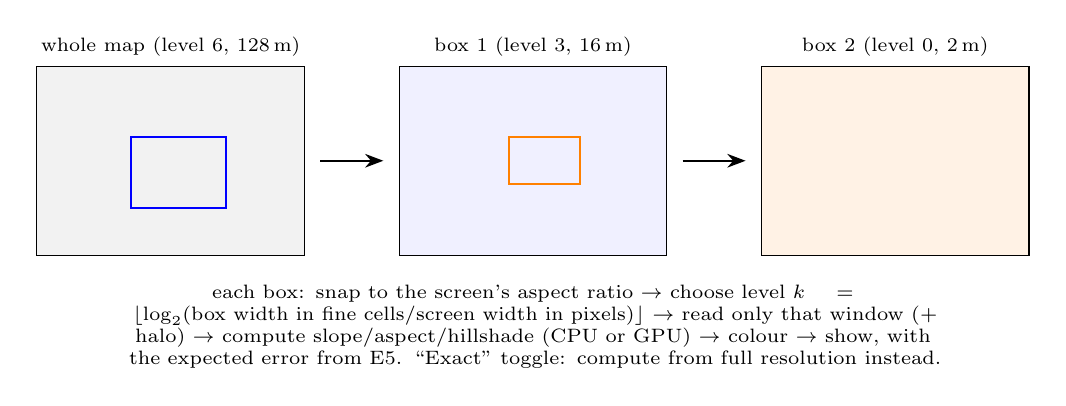
\begin{tikzpicture}[font=\small, arr/.style={-{Stealth}, thick}]
\draw[fill=gray!10] (0,0) rectangle (3.4,2.4); \node[font=\scriptsize] at (1.7,2.65) {whole map (level 6, 128\,m)};
\draw[thick, blue] (1.2,0.6) rectangle (2.4,1.5);
\draw[arr] (3.6,1.2) -- (4.4,1.2);
\draw[fill=blue!6] (4.6,0) rectangle (8.0,2.4); \node[font=\scriptsize] at (6.3,2.65) {box 1 (level 3, 16\,m)};
\draw[thick, orange] (6.0,0.9) rectangle (6.9,1.5);
\draw[arr] (8.2,1.2) -- (9.0,1.2);
\draw[fill=orange!10] (9.2,0) rectangle (12.6,2.4); \node[font=\scriptsize] at (10.9,2.65) {box 2 (level 0, 2\,m)};
\node[align=center, font=\scriptsize, text width=12.6cm, anchor=north] at (6.3,-0.25) {each box: snap to the screen's aspect ratio $\to$
choose level $k = \lfloor\log_2(\text{box width in fine cells} / \text{screen width in pixels})\rfloor$ $\to$ read only
that window (+ halo) $\to$ compute slope/aspect/hillshade (CPU or GPU) $\to$ colour $\to$ show, with the expected error from
E5. ``Exact'' toggle: compute from full resolution instead.};
\end{tikzpicture}
\caption{Box zoom: every step computes only the selected box, at the resolution the screen can show.}
\end{figure}
\textbf{Why this design:} explicit resolution handling, one computation per zoom step (easy to measure and to explain),
constant cost per view (E5), and a known accuracy cost shown to the user. \textbf{Choices made:} both a browser viewer
(native UTM, breadcrumb of boxes, back button, switches for operation / auto--exact / CPU--GPU) and a QGIS plugin (map
tool: drag a rectangle, the box comes back as a georeferenced layer), sharing one FastAPI server; automatic level with an
exact toggle; the XYZ tile server is dropped; the Cesium globe becomes a stretch item.

\textbf{Planned files:} \code{demlab/view.py} (box $\to$ level, window, compute, colour, PNG, timings; result cache),
\code{server/app.py} (\code{GET /overview}, \code{POST /view}, \code{GET /info}), \code{viz/web/}, \code{qgis\_plugin/},
\code{bench/experiments/e6\_view.py}.

\textbf{E6 will measure:} time per zoom step split into read, compute, colour map + PNG, transfer + display; p50/p95 over
random nested box sequences from the whole map to full resolution; CPU vs GPU; auto vs exact vs precomputed; cold vs warm;
result cache hit vs miss; QGIS drawing the same boxes as the baseline; expected slope error per step (from E5).

\subsection{Phase 6 (stretch) and Phase 7}
\textbf{Phase 6}, only if time allows: viewshed (exact R3 vs approximate XDraw vs \code{gdal\_viewshed}: time and share of
cells classified differently, gap G3; heights first converted to one vertical datum) and terrain distance (Dijkstra vs A*
on a slope-based cost surface). \textbf{Phase 7:} final report (introduction, literature, method, results E1--E6, the
bottleneck story, limitations), slides, live demo with a video fallback, code frozen and tagged.

\subsection{Schedule and owners (relative weeks)}
\noindent\begin{tabularx}{\linewidth}{lLl}
\toprule
When & Work & Owner (as in the plan) \\
\midrule
Weeks 1--2 & Phases 0--3 (setup, data, baseline, engine) & done \\
Weeks 2--3 & Phase 4 pyramid accuracy (E5) & done \\
Week 3 & Phase 5 box server + web viewer & Swayam \\
Week 3 & Phase 5 QGIS plugin (Cesium stretch) & Kartikeya \\
Week 3 & Phase 6 stretch, if on track & Siddharth \\
End of Week 3 & Report, slides, demo & all \\
\bottomrule
\end{tabularx}

\subsection{Open items}
\begin{itemize}
  \item The professor update (\code{docs/prof\_update\_phase2.md}) covers Phase 2 only and has not been sent; Phase 3 and 4
  progress reports are ready in \code{report/}.
  \item Possible improvements found but not done: cache decoded tiles across windows (halo re-decoding); a per-level
  correction factor for the slope underestimate; padding grids to a multiple of $2^k$ for exact overviews.
\end{itemize}

\subsection{Questions to ask the professor}
\begin{itemize}
  \item Is ``standard tools don't break, they become slow; after parallelising, data movement is the bottleneck'' the kind
  of bottleneck answer he wants, or should we also benchmark other tools (WhiteboxTools, GRASS)?
  \item Is box-based zoom acceptable as the interactive design (instead of continuous tile streaming)?
  \item Is an honest ``when the GPU helps and when it doesn't'' (1.4$\times$ end to end, 50$\times$ kernel) the expected GPU result?
  \item Is the slope underestimate at coarse levels acceptable for display, if the viewer shows the expected error?
\end{itemize}

%=====================================================================
\section{Presentation preparation}
\subsection{Numbers to remember}
\begin{tabularx}{\linewidth}{lL}
\toprule
Fact & Number \\
\midrule
Largest grid & 10.8 billion cells, 43\,GB float32, 2.6$\times$ RAM \\
gdaldem slope at 1\,m & 208\,s, 1 of 22 threads, 0.87\,GB RAM, 73\% computation \\
QGIS whole-area redraw at 1\,m & 31.9\,s without pyramid, 0.09\,s with (360$\times$) \\
Best storage layout & tiled ZSTD: 2.9$\times$ smaller, decodes 2.6$\times$ faster than LZW \\
Our CPU engine & 3.5$\times$ faster at 1\,m (60\,s), $\sim$1.4\,GB flat, identical to gdaldem \\
Naive whole-grid NumPy & $\sim$24\,B/cell, fails above $\sim$0.5--0.7\,B cells \\
Our GPU engine & 43.8\,s at 1\,m (4.75$\times$ gdaldem); kernel 50$\times$ CPU; copies 95\% of GPU time \\
GPU crossover & $512^2$ cells (slope), $256^2$ (three products) \\
Three products fused & 3.4--4.2$\times$ vs three gdaldem runs (CPU); 5.9$\times$ (GPU, 2\,m real) \\
On-demand tile & 5--8\,ms at every level; 8--450$\times$ faster than exact \\
Slope error per level & 2.3$^\circ$ (1 up), 4.4$^\circ$ (2), 5.6$^\circ$ (3), 6.4$^\circ$ (4), 10$^\circ$ (6); always too low \\
Aspect error & median 1.8--8.5$^\circ$ \\
Precomputed slope pyramid & 10.6\,s, 1.0\,GB per derivative \\
Runs measured & 1817 process runs (E1--E4) + E5 timings; 2 failures (intended out-of-memory) \\
\bottomrule
\end{tabularx}

\subsection{Suggested slide order}
\begin{enumerate}
  \item Problem and goal (MoM): big DEM, one laptop, find the real bottleneck, show only what is needed.
  \item Data: one area, real 90/30/8/2\,m + synthetic 2/1\,m; why synthetic is timing only.
  \item Method: harness, cold/warm, pinning, stage split; why it is fair.
  \item Baseline: gdaldem scaling, memory, stage split; QGIS with/without pyramid.
  \item Our engine: pipeline diagram; speed-up and memory; naive breaking point; correctness.
  \item GPU: kernel vs end to end; crossover; optimisation steps; ``the bottleneck moves'' chart.
  \item Pyramid on demand: error by level and slope class, maps, time saved, trade-off chart.
  \item The story and the answer to G1 and G2.
  \item Phase 5 box-zoom design (and demo, once built); limitations; future work.
\end{enumerate}

\subsection{Likely questions and answers}
\begin{longtable}{>{\raggedright\arraybackslash}p{5.2cm}>{\raggedright\arraybackslash}p{10.2cm}}
\toprule
Question & Answer \\
\midrule
\endhead
Why not just give gdaldem more threads? & We tested \code{GDAL\_NUM\_THREADS=ALL\_CPUS} and a 4\,GB cache: 2--4\% \emph{slower}. Only
decompression is parallel there; gdaldem's computation is single-threaded by design. \\
Is the comparison fair? & Same machine, grids, harness and cores (12 P-threads); gdaldem at its fastest settings; engine times
include Python start-up; results identical on every cell. \\
Why use upsampled 1\,m data? & No free 1\,m DEM exists for the area. Run time depends on cell count, which we verified on real vs
upsampled data; accuracy uses real data only. \\
Why is the GPU only 1.4$\times$ faster? & The kernel is 50$\times$ faster, but 95\% of the GPU's time is copying over PCIe and the
run is limited by decompressing and writing. Amdahl's law. \\
When does the GPU make sense? & Windows $\geq512^2$, several products at once, heavy operators, or results that stay in memory
(display), not written to disk. \\
Why does coarse-level slope come out lower? & Averaging smooths the terrain before the gradient is taken; steep, rough slopes lose
the most. \\
Is that error acceptable? & For display, yes (the map keeps every landform; error is shown). For thresholds (e.g.\ $>$45$^\circ$),
no: use the exact mode or a precomputed slope pyramid. \\
Why not precompute everything? & Exact and slightly faster, but a full pass and $\sim$1\,GB per derivative and parameter; on demand
needs no storage and supports any parameter. \\
Why bounding boxes instead of tiles? & Explicit resolution per step, one computation per zoom, constant cost, measurable, and the
error of each step can be shown. \\
How do you know your results are correct? & 119 tests; every cell of four full grids compared with gdaldem; differences explained
by gdaldem's float32 rounding and reproduced exactly. \\
How repeatable are the timings? & Median IQR 1.2--1.6\% of the median; cold cache verified; background interference detected and
removed; disturbed attempts kept as evidence. \\
What would change on another laptop? & Absolute times; the shape of the results (where the bottleneck is) should hold on similar
hardware; with a slow HDD, reading would matter more. \\
\bottomrule
\end{longtable}

%=====================================================================
\section{How to reproduce everything, and where things are}
\begin{verbatim}
conda activate geo
python datasets/prepare.py --synthetic            # rebuild all grids
powershell -ExecutionPolicy Bypass -File bench\run_phase2.ps1  # E1, E2, QGIS
powershell -ExecutionPolicy Bypass -File bench\run_e3.ps1      # E3 CPU
powershell -ExecutionPolicy Bypass -File bench\run_e4.ps1      # E4 GPU
python -m bench.experiments.e4_crossover
python -m bench.experiments.e5_timing --precompute
python -m bench.experiments.e5_accuracy
powershell -ExecutionPolicy Bypass -File bench\run_e5.ps1      # E5 timing
python -m pytest tests/ -q                                     # correctness
python -m tests.check_full_grid
python -m bench.analysis.phase2_report   # also: phase3_report,
                                         # e4_report, e5_report, run_stats
\end{verbatim}
\begin{tabularx}{\linewidth}{>{\raggedright\arraybackslash}p{6.4cm}L}
\toprule
Where & What \\
\midrule
\code{docs/PROJECT\_PLAN.md} & plan, methodology (\S6), phase status, Phase 5 design \\
\code{docs/PHASE2\_RESULTS.md}, \code{PHASE3\_RESULTS.md}, \code{PHASE3\_GPU\_RESULTS.md}, \code{PHASE4\_RESULTS.md} & detailed results per phase \\
\code{report/} & progress reports (Phase 2, 3, 4) and this report \\
\code{results/runs.csv}, \code{results/e5\_*.csv} & every measurement \\
\code{results/plots/}, \code{results/*\_tables.md}, \code{results/run\_stats.md} & charts, tables, spreads \\
\code{demlab/}, \code{bench/}, \code{tests/} & engine, harness and experiments, tests \\
\code{old files/} (local only) & earlier scripts, superseded results, logs, with a README \\
GitHub & \url{https://github.com/Swayamgoyal/Geoguessers} (no data, no \code{old files}) \\
\code{K:\textbackslash spatial project\textbackslash} \code{GeoGuessers\_handoff} & complete verified copy: project, all data,
environment, notes; start with \code{README\_HANDOFF.md} \\
\bottomrule
\end{tabularx}

\end{document}
